\documentclass{article}
\usepackage[utf8]{inputenc}
\usepackage{amsmath}
\usepackage{setspace}
\usepackage{mathtools}
\usepackage{amssymb}
\usepackage{amsfonts}
\newcommand\der[2]{\frac{\partial{#1}}{\partial{#2}}}
\usepackage{sectsty}
\usepackage[parfill]{parskip}
\usepackage{changepage}   % for the adjustwidth environment
\usepackage{graphicx}
\graphicspath{ {./Pictures/} }
\usepackage{float}
\usepackage[margin=1in]{geometry}
\setlength{\parindent}{0em}
\sectionfont{\fontsize{12}{12}\selectfont}
\nonfrenchspacing
\renewcommand{\baselinestretch}{1.5}
\usepackage{indentfirst}
\usepackage{enumitem}
\setlist[itemize]{topsep=0pt,itemsep=0pt,partopsep=0pt,parsep=0pt}
\usepackage{xcolor}
\usepackage{titlesec}
\DeclareUnicodeCharacter{2212}{-}
\usepackage{tikz}
\usetikzlibrary{calc}
\newcommand{\tikzmark}[1]{\tikz[overlay,remember picture] \node (#1) {};}
\titleformat{\section}[block]{\color{blue}\Large\bfseries\filcenter}{}{1em}{}
\usepackage[normalem]{ulem}

\title{Macroeconomics B Notes}
\author{Nicholas Umashev \footnote{content is not of my own authorship}}
\date{2019}

\begin{document}

\maketitle

\tableofcontents

\newpage

\section{Dynamic Optimization in Discrete Time}

\par \underline{Optimization Issues}: solving large problems (like that below is challenging using traditional methods and so we must rely on dynamic programming)
\begin{itemize}
    \item  \underline{Example}: consider the problem
    \begin{gather*}
        \max_{\{c_{t},k_{t+1}\}^{\infty}_{t=0}} \ \mathbb{E}_{0} \sum_{t=0}^{\infty} \beta^{t} \ln c_{t} \\ \text{subject to:} \ \ c_{t}+k_{t+1} \leq Ak_{t}^{\alpha}\theta_{t} \ \ \forall t, \ \ \ k_{0} \ \text{given}, \ \ \ \ln(\theta_{t}) \sim_{iid} N(0, \sigma^{2})
    \end{gather*}
    where $c_{t}$ is consumption, $k_{t}$ is capital, $\theta_{t}$ is a productivity shock
    \begin{itemize}
        \item  \underline{Issue}: this problem involves maximization over an infinite sequence of controls, subjects to an infinite sequence of constraints, and where each period's optimal decisions depend on the history of shocks and past decisions - making the problem more difficult
        \item \underline{Solution}: we are looking for a solution of the form $\{c_{t}^{*}(\theta^{t})\}_{t=0}^{\infty}$ and $\{k_{t}^{*}(\theta^{t})\}_{t=0}^{\infty}$ where $\theta^{t} = \{ \theta_{0}, \theta_{1}, \dots, \theta_{t} \}$ is the history of shocks up to $tS$
    \end{itemize}
\end{itemize}
\vspace{2.5mm}
\par \underline{Dynamic Programming}: breaks up optimization problems into a series of small and more tractable problems where the smaller problems are casted in a recursive way and are solved for a time-invariant policy function. Here the solution to such problems (under certain regularity conditions) can be used to recover the solution to the original problem
\begin{itemize}
    \item \underline{Bellman's Optimality Principle}: an optimal policy has the property that whwatever the initial state and initial decisions are, the remaining decisions must constitute an optimal policy with regard to the state resulting from the first decision.
    \begin{itemize}
        \item \underline{Note}: based on this principle the solution to the dynamic programming problem is a valid solution to the original problem
    \end{itemize}
    \item  \underline{Horizon Types}: can involve either finite horizon or infinite horizon problems
    \item  \underline{State Variables}: set of variables summarizing the state of the economy at each point in time
    \item  \underline{Control Variables}: the set of choice variables at each point in time
    \item  \underline{Value Function}: the optimal value of the original problem, given the states
    \begin{itemize}
        \item \underline{Note}:
    \end{itemize}
    \item  \underline{Policy Function}: the optimal value for the control variables, given the states
\end{itemize}
\vspace{2.5mm}
\par \underline{Primer on Dynamic Programming Concepts}: any optimization problem has some objective (such as minimizing cost) with the mathematical function that describes this objective being called the objective function. \\ \\
Dynamic programming breaks a multi-period planning problem into smaller steps at different points in time and therefore it requires keeping track of how the decision situation is evolving over time. The information about the current situation that is needed to make a correct decision is called the "the state". For example, to decide how much to consume and spend at each point in time, people would need to know their initial wealth and therfore wealth would be one of their state variables.\\ \\
The variables chosen at any given point in time are often called the "control" variables. For example, given their current wealth, people might decide how much to consume now. Choosing the control variables now may be equivalent to choosing the next state, since the next state is affected by the current control (in addition to other factors). For example, today's wealth (the state) and consumption (the control) might exactly determine tomorrow's wealth (the new state). \\ \\
The dynamic programming approach describes the optimal plan by finding a rule that tells what the control should be, given any possible value of the state. For example, if consumption $(c)$ depends only on wealth $(w)$ then we would seek a rule $c(w)$ that gives consumption as a function of wealth. Such a rule, determining the controls as a function of the states, is called a "policy function". \\ \\
Finally, the optimal decision rule is the one that achieves the best possible value of the objective. For example, if someone chooses consumption, given wealth, in order to maximize happiness (represented by a utility function), then each level of wealth with be associated with some highest possible level of happines $H(w)$. The best possible value of the objective, written as a function of the state, is called the value function. \\ \\
\vspace{1mm}
Therefore, a dynamic optimization problem in discrete time can be stated in a recursive, step-by-step, form known as backward induction by writing down the relationship between the value function in one period and the value function in the next period. The relationship between these two value functions is called the "Bellman Equation". In this approach, the optimal policy in the last time period is specified in advance as a function of the state variable's value at that time, and the resulting optimal value of the objective function is thus expressed in terms of that value of the state variable. \\ \\
Next, the next-to-last period's optimization involves maximizing the sum of that period's period-specific objective function and the optimal value of the future objective function, giving that period's optimal policy contingent upon the value of the state variable as of the next-to-last period decision. \\ \\
This logic continues recursively back in time, until the first period decision rule is derived, as a function of the initial state variable value, by optimizing the sum of the first-period-specific objective function and the value of the second period's value function, which gives the value for all the future periods. Thus, each period's decision is made by explicitly acknowledging that all future decisions will be optimally made.
\vspace{2.5mm}
\par \underline{Finite Horizon Problem}: consider a decision-maker solving the deterministic problem
\begin{gather*}
    \max_{\{ u_{t} \} _{t=0}^{T−1}} \sum_{t=0}^{T-1} \beta^{t}r(x_{t},u_{t}) + W(x_{T}) \\ \text{subject to:} \ x_{t+1} = g(x_{t}, u_{t}) \ \forall t, \ \ \ x_{0} \ \text{is given}
\end{gather*}
Here we assume a convex set, to ensure a maximum exists, and that the state space is discrete (ie $\mathcal{X} = \left\{x^{1}, x^{2}, \dots, x^{n}\right\}$). Our variables include:
\begin{gather*}
\beta \in (0,1): \ \text{the discount factor} \\
x \in \mathcal{X}:\ \text{the state variable} \\
u \in \mathcal{U}:\ \text{the control variable} \\
r(x_{t},u_{t}): \ \text{concave return function} \\
g(x_{t}, u_{t}): \ \text{the law of motion for the state} \\
W(x_{T}): \ \text{the terminal condition at} \ x_{t}
\end{gather*}
\begin{itemize}
    \item  \underline{Recursive Transformation}: based on the original problem being time separable we can write it as a series of recursive functions. The original problem asks us to find a sequence of $T$ controls (i.e. find $\{ u^{*}_{t} \}_{t=0}^{T-1}$) while the recursive formulation asks us to solve $T$ problems with one control each (i.e. find the series of $U_{t}^{*}(x)$ over the set $t$). \\ In other words, we transform the original problem of finding an infinite sequence of controls that maximizes our function for the problem of finding the optimal value function $V(x)$ and a function $h$ that solves the continuum of maximum problems (ie one maximum problem for each value of x). Here $h$ is a time-invariant policy function that maps the state $x_{t}$ into the control $u_{t}$ such that we can iteratively use $u_{t} = h(x_{t})$ and $x_{t+1} = g(x_{t}, u_{t})$ to find the sequence $\{u_{s}\}_{s=0}^{\infty}$
    We make the following Transformation
    \begin{gather*}
        \max_{\{u_{t}\}_{t=0}^{T−1}} \sum_{t=0}^{T−1} \beta^{t}r(x_{t},u_{t}) + W(x_{T}) \\
        \text{subject to:} \ x_{t+1} = g(x_{t},u_{t}) \ \forall t, \ \ \ x_{0} \ \text{is given} \\
        \Big\Downarrow \\
        V_{t}(x) = \max_{u} \left\{ r(x,u)+ \beta V_{t+1} (g(x, u)) \right\}
    \end{gather*}
    \item \underline{Value Function $V_{t}(x)$}: is the greatest feasible payoff from time $t$ forward if the state at time $t$ is $x_{t}$. Here the value function is
    \begin{gather*}
    V_{t}(x_{t}) = \max_{\{u_{s}\}_{s=t}^{T−1}} \sum_{s=t}^{T−1} \beta^{s}r(x_{s},u_{s}) + W(x_{T}) \\ \text{subject to}: \ x_{s+1} = g(x_{s}, u_{s}) \ \forall s, \ \ \ x_{t} \ \text{is given}
    \end{gather*}
    Note that this is different from our objective function in that the time starts at $t$ and not 0
    \begin{itemize}
        \item \underline{Bellman Condition}: given the structure of the problem, the value function satisfies the Bellman Equation. Here we want to solve for $V(x)$ and $h(x)$ together which are linked by the Bellman Equation:
        \begin{gather*}
            V_{t}(x) = \max_{u} \left\{ r(x,u) + \beta V_{t+1} (g(x, u)) \right\}
        \end{gather*}
        with the terminal condition $V_{T}(x) = W(x)$.
         \begin{itemize}
            \item  \underline{Intuition}: the value function at time $t$ is going to be the maximum utility given next period's value function, today's return, and the terminal condition. Note that the Bellman Equation describes the value function, at a given point in time, as a function of itself in another point in time. Note that the maximizer of the Bellman equation is a policy function $h(x)$ (also notated as $U_{t}(x)$) that satisfies $$V(x) = r[x, h(x)] + \beta V \left\{g[(x, h(x)] \right\}$$
         \end{itemize}
    \end{itemize}
    \item  \underline{Policy Function $U_{t}(x)$}: the policy function describes the utility that, given the state, is the maximum of the value function. In other words, the maximizer of the RHS of the bellman equation is a policy function $h(x)$. Given $V_{t}(x)$, we define the policy function by
    \begin{gather*}
        U_{t}(x) = \arg \max_{u} \left\{ r(x,u) + \beta V_{t+1} (g(x, u)) \right\}
    \end{gather*}
    \item \underline{Assumptions}: in order to solve the Bellman Equation we need to impose the following assumptions
    \begin{itemize}
        \item  \underline{Assuumption 1}: the Bellman Equation has a unique strictly concave solution
        \item  \underline{Assumption 2}: the solution is approached in the limit as $j \rightarrow \infty$ by iterations on
        \begin{gather*}
            V_{j+1}(x) = \max_{u} \left\{r(x,u) + \beta V_{j}(\widetilde{x}) \right\}
        \end{gather*}
        Subject to $\widetilde{x} = g(x,u)$, $x$ given, and starting from any bounded and continuous initial $V_{0}$. Note that $\widetilde{x}$ is tomorrows $x$
        \item  \underline{Assumption 3}: there is a unique and time-invariant optimal policy of the form $u_{t} = h(x_{t})$, where $h$ is chosen to maximize the RHS of the Bellman equation
        \item  \underline{Assumption 4}: off the corners, the limiting value function $V$ is differentiable
    \end{itemize}
    \item  \underline{Solution}: the Bellman Equation and the Policy Function are the building blocks for constructing the optimal solution
    \begin{itemize}
        \item  \underline{Step 1 - Backward Induction}: compute $\{ V_{t} (x) \}_{t=0}^{T}$ and $\{ U_{t} (x) \}_{t=0}^{T−1}$ by backward induction using the Bellman Equation
        \begin{itemize}
            \item \underline{Part 1}: compute $V_{t}(x) = W(x) \ \forall x \in \mathfrak{X}$
            \item  \underline{Part 2}: for all $t = T − 1, T −2, \dots, 0$ compute $V_{t}(x) = \max_{u} \{ r(x,u) + \beta V_{t+1} (g(x, u)) \}$ and $U_{t}(x) = \arg \max_{u} \{ r(x,u) + \beta V_{t+1} (g(x, u)) \}$ for all $x \in \mathcal{X}$
            \item \underline{Example}
            \begin{gather*}
                \boxed{t=T} \\
                \forall x^{i}, \ \begingroup\color{magenta} V_{T}(x^{i}) \endgroup = W(x^{i}) \rightarrow \ \text{final condition} \\
                \\
                \boxed{t=T-1} \\
                \forall x^{i}, \ V_{T-1}(x^{i}) = \max_{u} \left\{ r(x^{i}, u) + \beta \begingroup\color{magenta} V_{T}(x^{i}) \endgroup \right\} \\
                U_{T-1}(x^{i}) = \arg \max_{u} \left\{ r(x^{i}, u) + \beta V_{T}(x^{i}) \right\} \\
                \dots \\
                \text{repeat these steps until we reach} \ \boxed{t=0}
            \end{gather*}
            Note that because the state variable x is discrete, we know how many times we need to iterate backwards until $t=0$
        \end{itemize}
        \item  \underline{Step 2 - Iterating Forward}: given $x_{0}$ compute $\{u_{t}^{*}\}_{t=1}^{T−1}$ and $\{x_{t}^{*}\}_{t=1}^{T}$ by iterating forward on $$\{ U_{t} (x) \}_{t=0}^{T−1}$$
        \begin{itemize}
            \item \underline{Method}: we iterate forward using $x$
            \begin{gather*}
                u_{0}^{*} = U_{0}(x_{0}^{*}), \ \ \tikzmark{a}x_{1}^{*} = g(x_{0}^{*}, u_{0}^{*}), \\
                u_{1}^{*} = U_{1}(x\tikzmark{b}_{1}^{*}), \ \ x_{2}^{*} = g(x_{1}^{*}, u_{1}^{*}), \\
                \dots \\
                u_{t}^{*} = U_{t}(x_{t}^{*}), \ \ x_{t+1}^{*} = g(x_{t}^{*}, u_{t}^{*}), \\
                \dots \\
                u_{T-1}^{*} = U_{T-1}(x_{T-1}^{*}), \ \ x_{T}^{*} = g(x_{T-1}^{*}, u_{T-1}^{*}),
                \begin{tikzpicture}[overlay,remember picture,-latex,shorten >=0.001pt,shorten <=0.001pt]
                    \draw[->,red, distance=0.25cm] (a.south) to (b.north west);
                \end{tikzpicture}
            \end{gather*}
            \item \underline{Intuition}: the law of motion will indicate what the future value of $x_{t}$ is given the control variable $u$, allowing us to derive the solution. Note that the control variable $u$ is able to be calculated due to having previously found the value of $u$ via backward induction in step 1
        \end{itemize}
    \end{itemize}
\end{itemize}
\vspace{2.5mm}
\par \underline{Infinite Horizon Problem}: consider the problem \begin{gather*}
\max_{\{u_{t}\}_{t=0}^{\infty}} \ \sum_{t=0}^{\infty} \beta^{t}r(x_{t}, u_{t}) \\
\text{subject to}: \ x_{t+1} = g(x_{t}, u_{t}), \ \ \ x_{0} \text{is given}
\end{gather*}
We want to compute the solution $\{u_{t}^{*}, x_{t+1}^{*}\}_{t=0}^{\infty}$
\begin{itemize}
    \item \underline{Assumptions}: in addition to the previous finite horizon problem assumptions we assume that $r(\cdot)$ is bounded, also note that now the bellman equation is a functional equation in V
    \item  \underline{No Backward Induction}: since there is no terminal condition to start with (ie V is time-invariant) we cannot use backward induction
    \item \underline{Conditions for a Solution}: the following four conditions must hold for the infinite horizon problem to be solved
    \begin{itemize}
        \item \underline{Condition 1}: the Bellman Equation has a unique strictly concave solution $V^{*}$
        \item \underline{Condition 2}: let $V^{0}$ be any bounded and continuous VF and let $V^{j}$ satisfy
        \begin{gather*}
            V^{j}(x) = \max_{u} \left\{ r(x,u) + \beta V^{j-1}(g(x,u)) \right\} \ \ \text{for} \ j \geq 1
        \end{gather*}
        Then $V^{*} = \lim_{j \rightarrow \infty} V^{j}$
        \item \underline{Condition 3}:There is a unique and time-invariant policy function $U^{*}$ such that the solution to the original problem can be obtained by iterating on $u^{*}_{t} = U^{*}(x_{t})$
        \item \underline{Condition 4}: off the corners, the limiting value function $V^{*}$ is differentiable with
        \begin{gather*}
            V^{*'}(x) = r_{1}(x, U(x)) + \beta V^{*'}(g(x,U(x)))g_{1}(x,U(x))
        \end{gather*}
    \end{itemize}
    Note that the second condition implies that if you have any function $V_{0}$ that is bounded and continuous then if you iterate on $j$ you will eventually find the solution $V^{*}$ (ie a steady state). The third condition implies that from finding $V^{*}$ you can use $u_{*}$ to then backwards iterate to find $U^{*}$
    \item  \underline{Guess and Verify Method}: also known as the method of undetermined coefficients, this involves guessing and verifying a solution $V$ to the Bellman Equation. This relies on the uniqueness of the solution to the Bellman Equation (condition 1) and can be solved analytically with pen and paper (though does not always work)
        \begin{itemize}
            \item  \underline{Step 1}: guess that the true value function has a particular parametric form $V^{G}(x; A)$ where A is a vector of unknown parameters
            \item  \underline{Step 2}: compute $\widehat{V}(x;A) = \max_{u} \{r(x,u) + \beta V^{G}(g(x,u);A) \}$
            \begin{itemize}
                \item \underline{Note}: you can solve for the control variable that is implied by the policy function by using the FOC (provided in condition 4). This then allows you to solve for the optimized $\widehat{V}(x;A)$
            \end{itemize}
            \item  \underline{Step 3}: if there exists parameters $A^{*}$ such that $\widehat{V}(x; A^{*}) = V^{G}(x;A^{*})$ then $V^{G}(x;A^{*})$ is the solution
            \begin{itemize}
                \item \underline{Note}: compare the derived optimized value function $\widehat{V}(x;A)$ from step 2 to $V^{G}(x; A)$
            \end{itemize}
        \end{itemize}
    \item \underline{Value Function Iteration Method}: we proceed by constructing a sequence of value functions and associated policy functions. The sequence is created by iterating on the following equation, starting from $V_{0} = 0$, and continuing until $V_{j}$ has converged:
    \begin{gather*}
        V_{j+1}(x) = \max_{u} \left\{r(x,u) + \beta V_{j} (\widetilde{x}) \right\} \\
        \text{subject to} \ \ \ \widetilde{x} = g(x,u), \ x \ \ \text{given}
    \end{gather*}
     This method always works because by solution method condition 2 we have $V^{*} = \lim_{j \rightarrow \infty} V^{j}$, however this method can be very slow particularly for problems with more than one state
    \begin{itemize}
        \item  \underline{Step 1}: start from any bounded and continuous guess $V^{0}$
        \item  \underline{Step 2}: iterate on $V^{j}(x) = \max_{u} \{ r(x,u) + \beta V^{j−1} (g(x,u)) \}$ until convergence (ie until $||V^{j} − V^{j−1}|| < \varepsilon$)
    \end{itemize}
    \item  \underline{Policy Function Iteration Method}
    \begin{itemize}
        \item  \underline{Step 1}: pick a feasible policy function $U^{0}(x)$ (or $u = h_{0}(x)$) and compute the value associated with operating forever with that policy
        \begin{gather*}
            V_{h_{j}}(x) = \sum_{t=0}^{\infty} \beta^{t} r [x_{t}, h_{j}(x_{t})]
        \end{gather*}
        where $x_{t+1} = g[x_{t}, h_{j}(x_{t})]$ with $j=0$
        \item  \underline{Step 2}: generate a new policy $u = h_{j+1}(x)$ that solves the two period problem
        \begin{gather*}
            \max_{u} \left\{r(x,u) + \beta V_{h_{j}} [g(x,u)]\right\}
        \end{gather*}
        for each x
        \item  \underline{Step 3}: iterate over j until convergence, repeating steps 1 and 2
    \end{itemize}
    \item  \underline{Example}: consider a social planner solving
    \begin{gather*}
    \max_{\{c_{t}, k_{t+1} \}_{t=0}^{\infty}} \ \sum_{t=0}^{\infty} \beta^{t} \ln (c_{t}) \\
    \text{subject to}: \ c_{t} + k_{t+1} = Ak_{t}^{\alpha}, \ \ \ k_{0} \ \text{is given}
    \end{gather*}
    where $\alpha \in (0,1)$ and $\beta \in (0,1)$
    \begin{itemize}
        \item \underline{Simplification}: rearranging the constraint and substituting $$c_{t}$$ into the objective function we have
        \begin{gather*}
        \max_{\{k_{t+1} \}_{t=0}^{\infty}} \ \sum_{t=0}^{\infty} \beta^{t} \ln (Ak_{t}^{\alpha} − k_{t+1}) \\
        \text{subject to}: \ k_{0} \ \text{is given}
        \end{gather*}
        Here the State Variable is $t \rightarrow k^{t}$ (i.e. today's capital) and the control variable is $t \rightarrow k_{t+1}$ (i.e. tomorrow's capital). Note that indexes have been dropped since it is an infinite horizon problem with k being the state and k' being the control. The Bellman Equation given this simplication is
        \begin{gather*}
            V(k) = \max_{k^{'}} \{ \ln(Ak^{\alpha} − k^{'}) + \beta V(k^{'}) \}
        \end{gather*}
        \item  \underline{Guess and Verify Solution}: here we guess the functional form $V^{G}(k; E, F) = E + F \ln (k)$ where E and F are unknown constants. We then plug in $V^{G}(x; E, F)$ into the RHS of the Bellman equation yielding
        \begin{gather*}
            \widehat{V}(k; E, F) = \max_{k} \Big\{ \ln(Ak^{\alpha} - k^{'}) + \beta V^{G}(k^{'}; E, F) \Big\} = \max_{k} \Big\{ \ln(Ak^{\alpha} - k^{'}) + \beta(E + F \ln (k)) \Big\}
        \end{gather*}
         Taking first order conditions and log-linearizing results in the optimal policy function $k^{'}(k) = \frac{\beta F}{1 + \beta F}Ak^{\alpha}$. Substituting the optimal policy function into the objective function yields
         \begin{gather*}
             \widehat{V}(k;E,F) = \underbrace{\bigg[ \ln \Big(\frac{A}{1+\beta F} \Big) + \beta F \ln \Big( \frac{\beta F}{1 + \beta F} A \Big) + \beta E \bigg]}_{E^{'}} + \underbrace{\alpha(1+\beta F) \ln(k)}_{F^{'}} \\
             \Updownarrow \\
             \widehat{V}(k; E^{'}, F^{'}) = E^{'} + F^{'} \ln(k)
         \end{gather*}
         When grouping the constants for $\widehat{V}(k; E’, F’)$ it has the same functional form as $V^{G}(k; E, F)$. Finally, we pin down the unknown coefficients by solving the system of equations
         \begin{align*}
             E^{*} &= \bigg[ \ln \Big(\frac{A}{1+\beta F} \Big) + \beta F \ln \Big( \frac{\beta F}{1 + \beta F} A \Big) + \beta E \bigg] \\
             F^{*} &= \alpha(1+\beta F) \ln(k)
         \end{align*}
         Note that the equation for $E^{*}$ is derived from collecting constant terms and $F^{*}$ is derived from collecting the terms containing our dependent variable. This leaves us with the final solution $V^{*} = E^{*} + F^{*} \ln (k)$ and the optimal policy function $k^{'*}(k) = \frac{\beta F^{*}}{1 + \beta F^{*}} A k^{\alpha}$
         \begin{itemize}
             \item \underline{Solution Write Out}: here the Bellman Equation is $V(k) = \max_{k^{'}} \left\{ \ln(A k^{\alpha} - k^{'}) + \beta V(k^{'}) \right\}$
             \begin{itemize}
                 \item  \underline{Step 1}: my guess is $V^{G} (k) = F \ln (k) + E$ where $F$ and $E$ are our unknown constants
                 \item  \underline{Step 2}: using my guess we have
                 \begin{gather*}
                     \widehat{V}(k) = \max_{k^{'}} \Big\{ \ln(Ak^{\alpha} - k’) + \beta (Ak^{\alpha} - k’) \Big\} = \max_{k^{'}} \Big\{ \ln(Ak^{\alpha} - k^{'}) + \beta(E + F \ln (k^{'})) \Big\}
                 \end{gather*}
                 Taking first order conditions we have the following
                 \begin{gather*}
                    -\frac{1}{Ak^{\alpha}-k^{'}} + \beta F \frac{1}{k^{'}} = 0 \\
                    \Downarrow \\
                    k^{'} = \frac{\beta F}{1 + \beta F} Ak^{\alpha} \tag{$\star$}
                 \end{gather*}
                 Plugging $\star$ into the objective function, we obtain the optimized value function $\widehat{V}(k)$
                 \begin{gather*}
                     \widehat{V}(k;E,F) = \underbrace{\bigg[ \ln \Big(\frac{A}{1+\beta F} \Big) + \beta F \ln \Big( \frac{\beta F}{1 + \beta F} A \Big) + \beta E \bigg]}_{E^{'}} + \underbrace{\alpha(1+\beta F)}_{F^{'}} \ln(k)
                 \end{gather*}
                 \item  \underline{Step 3}: to evaluate the parameters $(E^{*}, F^{*})$ we solve the system of equations implied by the functional form
                 \begin{align*}
                     \widehat{V}(k) &= E^{'} + F^{'} \ln (k) \\
                     V^{G}(k) &= E + F \ln(k)
                 \end{align*}
             This yields
                 \begin{align*}
                     E^{'} = E &\Rightarrow E = \ln \Big(\frac{A}{1+\beta F} \Big) + \beta F \ln \Big( \frac{\beta F}{1 + \beta F} A \Big) + \beta E \\
                     F^{'} = F &\Rightarrow F = \alpha(1+\beta F)
                 \end{align*}
                 Note that by $F = \alpha(1+\beta F)$ and $F^{'} = F$ we have $F^{*} = \tfrac{\alpha}{1 - \alpha \beta}$ which gives us the policy function with one unknown $k^{'*}(k) = \tfrac{\beta F^{*}}{1 + \beta F^{*}} A k^{\alpha}$
             \end{itemize}
         \end{itemize}
    \end{itemize}
\end{itemize}
\vspace{2.5mm}
\par \underline{Stochastic Problems}: consider the stochastic problem
\begin{gather*}
\max_{\{ u_{t} \} ^{\infty}_{t=0}} \mathbb{E}_{0} \sum_{t=0}^{\infty} \\
\text{subject to}: \ x_{t+1} = g(x_{t}. U_{t}, \varepsilon_{t+1}), \ \ \ \text{given} \ x_{t}
\end{gather*}
\begin{itemize}
    \item  \underline{iid Shocks}: $\varepsilon_{t}$ is a sequence of iid shocks with the cumulative distribution function $\Pr [\varepsilon_{t} \leq e ] = F(e)$
    \begin{itemize}
        \item \underline{Timing}: $\varepsilon_{t+1}$ is realized at $t+1$ after $u_{t}$ has been chosen, therefore $x_{t}$ is a sufficient statistic at $$t$$
        \item \underline{iid Assumption}: this is important for recursive formulation for if shocks were persistent instead then the state vector should also incorporate past shock realizations
    \end{itemize}
    \item \underline{Bellman Equation}: the Bellman Equation for this problem is
    \begin{gather*}
        V(x) = \max_{u} \{ r(x,u) + \beta \mathbb{E}[V(g(x,u, \varepsilon))|x] \}
    \end{gather*}
    where $\mathbb{E} [V(g(x, u, \varepsilon))|x ] = \int V(g(x,u,\varepsilon))dF(\varepsilon)$ and $V(x)$ is the optimal value of the problem starting from $x$ at $t=0$
    \item \underline{Solution Methods}: the previous solution methods still apply and the solution $V(x)$ of the Bellman Equation can be computed by iterating on
    \begin{gather*}
        V_{j+1}(x) = \max_{u} \left\{r(x,u) + \beta \mathbb{E} \bigg[ V_{j}[g(x,u,\varepsilon) | x] \bigg] \right\}
    \end{gather*}
    starting from any bounded continuous initial $V_{0}$.
    The first order necessary condition for the problem on the RHS of the Bellman Equation is
    \begin{gather*}
        r_{2}(x,u) + \beta \mathbb{E} \left\{V^{'} [g (x, u, \varepsilon)] g_{2}(x,u,\varepsilon) | x \right\} = 0
    \end{gather*}
    which we obtain simply by differentiating the Bellman Equation and passing the differentiation operation under the $\mathbb{E}$ (an integration) operator. Off corners, the value function satisfies
    \begin{gather*}
        V^{'}(x) = r_{1}[x, h(x)] + r_{2}[x, h(x)]h^{'}(x) + \beta \mathbb{E}\left\{ V^{'} \{g [x, h(x), \varepsilon] \} \{g_{1}[x,h(x), \varepsilon] + g_{2}[x, h(x), \varepsilon]h^{'}(x) \} | x \right\}
    \end{gather*}
    When the states and controls can be defined in such a way that $x$ does not appear in the transition equation, the formula for $V^{'}$ becomes
    \begin{gather*}
        V^{'}(x) = r_{1}[x, h(x)]
    \end{gather*}
    Substituting this formula into the first order necessary condition for the problem gives the stochastic Euler equation
    \begin{gather*}
        r_{2}(x,u) + \beta \mathbb{E} [r_{1}(\widetilde{x}, \widetilde{u})g_{2}(x, u, \varepsilon) | x] = 0
    \end{gather*}
    where tildes over $x$ and $u$ denote next period values.
    \begin{itemize}
        \item \underline{Integral Valuation}: the integral in expectation can be approximated by quadrature, if closed form solutions are infeasible
    \end{itemize}
\end{itemize}

\newpage

\section{Dynamic Optimisation in Continuous Time}

\par \underline{\bf{Continuous vs Discrete Time}}: in discrete time the intervals between periods are $\Delta>0$ (e.g. the interval between $t$ and $t+1$ is 1), in continuous time the intervals between periods are $\Delta \rightarrow 0$
\begin{itemize}
    \item  \underline{Continuous Variables Issue}: while state variables are often naturally continuous, when using computational methods we can only evaluation the value function  on a finite number of points. Since continuous variables are not countable this becomes an issue
    \begin{itemize}
        \item \underline{Solution}: we can address this problem via using (1) discretization of the state space, or, (2) polynomial approximation to the value function
    \end{itemize}
\end{itemize}
\vspace{2.5mm}
\par \underline{\bf{Discretization Method}}: consider a problem with continuous state and control variables $\mathfrak{x} \in \mathbb{R}$, discretization just replaces $\mathfrak{x}$ and $\mathfrak{u}$ by the finite grids $\widehat{\mathfrak{x}} = \{ x^{1}, \dots, x^{n} \}$ and $\widehat{\mathfrak{u}} = \{ u^{1}, \dots, u^{n} \}$. Here we discretize for a vector of unknown capital levels $k = [0, k_{1}, \dots, \overline{k}]$, we need to decide how big of a grid should we create when discretizing
\begin{itemize}
    \item \underline{Value Function Impact}: now the value function becomes a finite list of numbers, $V = [V^{1}, \dots, V^{n}]^{T}$
    \item  \underline{Advantage}: the maximization step is much simpler than under the original bellman equation, which is a key advantage of discretization methods
    \item  \underline{Disadvantage}: there is a "curse of dimensionality" in muiltidimensional state spaces where we can have either $N$ points for a one-dimensional state space vs $N^{k}$ points for a k-dimensional state space, which increases the number of states.
    \begin{itemize}
        \item  \underline{Grid Decision}: requires some a-priori information about the state space, which is sometimes difficult to obtain (e.g. upper and lower bounds). Typically, you choose a steady state level of capital and then select the grid up to that steady state
    \end{itemize}
    \item  \underline{Optimal Growth Illustration}: suppose $V(k) = \max_{k'} \left\{ \ln (Ak^{\alpha} - k') + \beta V(k') \right\}$ where in this case $\mathfrak{x} = \mathfrak{u}$
    \begin{itemize}
        \item \underline{Discretization}: if we discretize $\mathfrak{x}$ then the Bellman equation becomes $V_{i} = \max_{j} \left\{ \ln (Ak^{\alpha}_{i} - k_{j}) + \beta V_{j} \right\}$ for all $i = 1, \dots, n$ where $i$ indexes the different possible current levels of capital and $j$ indexes the different possible levels of future capital
        \item \underline{Value Function Iteration Illustration}: suppose we applied value function iteration and therefore iterate on the mapping $V_{i}^{s} = \max \left\{ \ln(Ak^{\alpha}_{i} - k_{1}) + \beta V_{1}^{s-1}, \dots, \ln(Ak_{i}^{\alpha} - k_{n}) + \beta V_{n}^{s-1} \right\}$ for all $i = 1, \dots, n$ where $s$ indexes the iteration step
        \begin{itemize}
            \item \underline{Step 1}: start with a guess
            \begin{gather*}
                v_{n \times 1}^{0} = \begin{bmatrix} v_{1}^{0} \\ v_{2}^{0} \\ \dots \\ v_{n}^{0} \end{bmatrix}, \ \ \ \text{where} \ \ v_{i}^{0} \equiv v^{0}(k_{i})
            \end{gather*}
            Note that our guess on $V^{0}$ has a dimension of $N \times 1$ which is the vector of all values of $v_{0}$ given different levels of capital. Therefore you have $N \times 1$ guesses
            \item \underline{Step 2}: find $V^{1}$ by solving $V_{i}^{1}=\max_{j} \left\{ \ln(Ak_{i}^{\alpha} - k_{j}) + \beta V_{j}^{0} \right\}$ where
            \begin{gather*}
                V_{i}^{1} = \max \begin{bmatrix} \ln(Ak_{i}^{\alpha} - k_{i}) + \beta V_{1}^{0} \\ \ln(Ak_{i}^{\alpha} - k_{2}) + \beta V_{2}^{0} \\ \dots \\ \ln(Ak_{i}^{\alpha} - k_{n}) + \beta V_{n}^{0} \end{bmatrix} \ \ \ \forall i, \ \ \ \text{which reduces to} \ \ \ V_{n \times 1}^{1} = \begin{bmatrix} V_{1}^{1} \\ V_{2}^{1} \\ \dots \\ V_{n}^{1} \end{bmatrix}
            \end{gather*}
            \begin{itemize}
                \item \underline{Note}: $V_{j}^{1}$ is the maximum element contained in the  $N \times 1$ vector of $v_{n \times 1}^{1}$'s. Note that this involves just picking the maximum possible element in the $v_{i}^{1}$ vector containing every possible level of capital for today (ie period $i$)
            \end{itemize}
            \item \underline{Step 3}: check for convergence, setting the tolerance level to the euclidean norm
            \begin{itemize}
                \item \underline{Tolerance Level($\varepsilon$)}: $||v^{1} - v^{0}||< \varepsilon$ where $\varepsilon = \sqrt{\sum_{i=1}^{n}(v_{i}^{1}-v_{i}^{0})}$
            \end{itemize}
            \item  \underline{Step 4}: compute $v^{s}$ by solving $v_{i}^{s} = \max \left\{ \ln(Ak_{i}^{\alpha} - k_{j}) + \beta v_{j}^{s-1} \right\} \ \ \ \forall i$
            \item  \underline{Step 5}: check convergence $||v^{s} - v^{s-1}||< \varepsilon$, if convergence holds then stop else go back to step 2 and iterate again
        \end{itemize}
    \end{itemize}
\end{itemize}
\vspace{2.5mm}
\par \underline{\bf{Ordinary Differential Equations (ODEs)}}: a "differential" equation" is one where the unknown is a function (instead of a variable) and the equation includes one or more of the derivatives of the function, an "ordinary differential equation" equation is one for which the unknown is a function of only one variable (typically time). The order of an ODE is that of the highest derivative - i.e. if the highest derivative is an ODE of order n then it is an nth-order ODE. The goal when solving an ODE is to find the behaviour of of the equation with respect to the unknown (i.e. how it evolves with time)
\begin{itemize}
    \item \underline{Partial ODEs}: where the unknown is a function of more than one variable
    \item  \underline{First-Order ODE Form}: $\dot{x}(t) = F(t, x(t))$, where $\dot{x}(t) \equiv dx(t)/dt$ and $t \in [t_{a}, t_{b}]$
    \begin{itemize}
        \item \underline{Unknown}: here the unknown is a function $x(t)$ with $x: [t_{a}, t_{b}] \rightarrow \mathbb{R}$ and can be found (without uniqueness) by integrating and combining with a initial condition
        \item  \underline{Uniqueness}: the solution is not unique with the form having infinitely many solutions indexed by an integrating constant C. However, generally the constant C can be uniquely determined by requiring the solution to pass through a given point on the $x(t)$-plane, providing us with a general and particular solution
        \item  \underline{Example}: $\dot{x}(t) = 2t$ with $t \in [0,\infty)$ where the dot on top of $x(t)$ represents the derivative of $x(t)$ with respect to time
        \begin{itemize}
            \item \underline{Solution without Initial Condition}: the general solution is $x(t) = t^{2} + C$
            \item  \underline{Solution with Initial Condition}: suppose we impose the initial condition $x(0) = 1$, therefore $C=1$ and the particular solution is $x(t) t^{2} + 1$
            \newline
            \begin{center}
            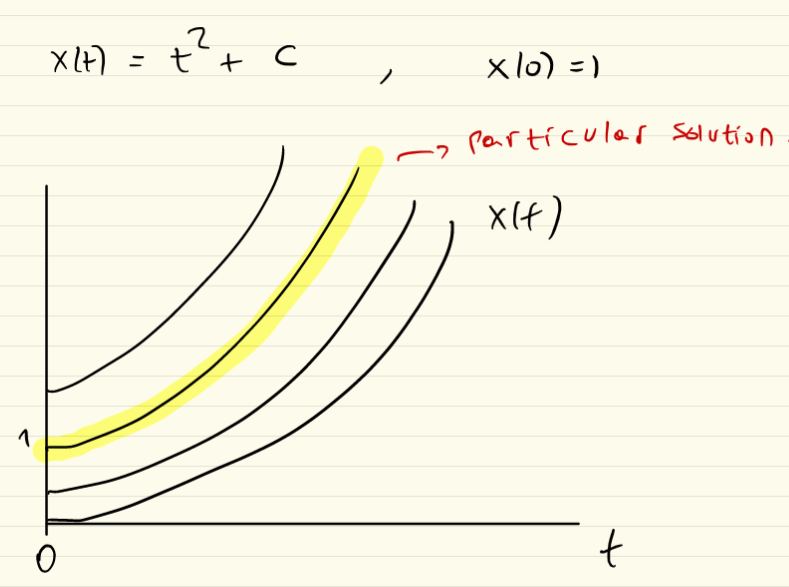
\includegraphics[width=4cm, height=3cm]{pic5}
            \end{center}
        \end{itemize}
    \end{itemize}
    \item  \underline{Finite-Difference Methods for Solution}: here we approximate derivates using finite-differences to approximate the solution to the ODE. This involves finding $\dot{x}(t) = F(t,x(t))$, $x(t_{a}) = x_{a}$, and $t \in [t_{a}, t_{b}]$. There are a wide range of methods depending on how the derivatives are approximated
    \begin{itemize}
        \item  \underline{Euler's Method}: given the equation implied by the ODE
        \begin{itemize}
            \item  \underline{Step 1}: specify a grid for t, i.e. $t_{0} = t_{a} < t_{1} < t_{2} < \dots < t_{N} = t_{b}$
            \item  \underline{Step 2}: we can approximate the ODE using the difference equation $$\frac{x(t_{i+1}) - x(t_{i})}{t_{i+1}-t_{i}} = F(t_{i},x(t_{i}))$$ iterating over $i = 0, \dots, N-1$, where $x(t_{0})=x_{a}$ is fixed by the initial condition
                \begin{itemize}
                    \item  \underline{Note}: the difference equation is obtained by rearranging the equation in step 1, we know all elements on the RHS of the difference equation which provides us with an explicit solution for $x(t_{1})$
                \end{itemize}
        \end{itemize}
        \item  \underline{Euler's Method Illustration}:
        \begin{itemize}
            \item  \underline{Step 1}: discretize $[t_{a}, t_{b}]$
            \item  \underline{Step 2}: iterate forward on $x(t_{i_1}) = x(t_{i}) + (t_{i+1} - t_{1})F(t_{i}, x(t_{i})) \ \ \ \forall i$
            \begin{itemize}
                \item \underline{i=0}: $x(t_{1}) = x(t_{0}) + (t_{1} - t_{0})F(t_{0}, x(t_{0}))$
                \item  \underline{i=1}: $\dots$ (etc)
            \end{itemize}
        \end{itemize}
        \item  \underline{Euler's Method Numerical vs Analytical Solution Equivalency}: $\dot{x}(t) = 2t, \ \ x(0)=1, \ \ t \in [0, 1000]$
            \newline
            \begin{center}
            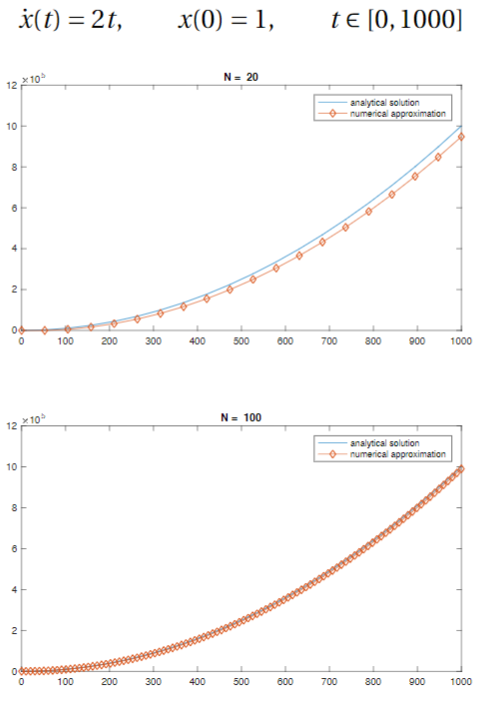
\includegraphics[width=5cm, height=3cm]{pic6}
            \end{center}
    \end{itemize}
    \item \underline{ODE Systems}: consider the system of two equations in two unknowns
    \begin{gather*}\dot{x}(t) = f(t, x(t), y(t)) \\ \dot{y}(t) = g(t, x(t), y(t)) \end{gather*} where $t \in [t_{a}, t_{b}]$. The general solution typically depends on two arbitrary constants,  say A and B, and can be written as \begin{gather*} x(t) = \phi_{1} (t; A, B) \\ y(t) = \phi_{2} (t; A,B) \end{gather*} Here the two arbitrary constants  A and B can be pinned down via two conditions on the solution which causes two types of problems emerge. In other words, the function must be solved such that both the initial and boundary conditions hold. Note that, like single-equation ODEs, exact solutions ODE systems can only be obtained under special cases
    \begin{itemize}
        \item \underline{Initial Value Problem(IVP)}: where you have conditions on the initial time ($a$) values - here $x(t_{a}) = x_{a}$, $y(t_{a}) = y_{a}$ can be solved numerically by applying Euler's Methods
        \begin{itemize}
            \item \underline{Step 1}: discretize the domain
            \item  \underline{Step 2}: iterate forward starting from $x(t_{a}) = x_{a}$ and $y(t_{a}) = y_{a}$
        \end{itemize}
        \item  \underline{Boundary Value Problem (BVP)}: where you have a condition on the value at a time period ($b$) that different from the initial time value ($a$) - here $x(t_{a}) = x_{a}$, $y(t_{b}) = y_{b}$ can be solved by applying a shooting algorithm
        \begin{itemize}
            \item \underline{Step 1}: make an initial guess for $y(t_{a})$ called $y_{a}^{G}$
            \item \underline{Step 2}: solve the ODE system by applying Euler's method given $x(t_{a}) = x_{a}$ and $y(t_{a}) = y_{a}^{G}$
            \item \underline{Step 3}: if $y(t_{b})$ is 'close enough' to $y_{b}$ then stop, else update $y_{a}^{G}$ and go back to step 2
            \newline
            \begin{center}
            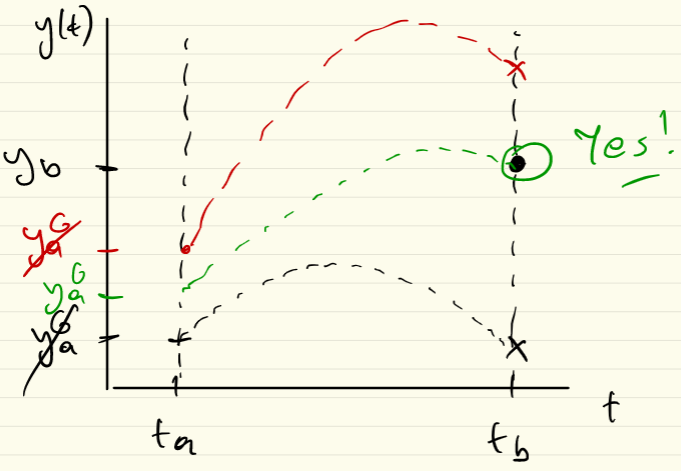
\includegraphics[width=4cm, height=3cm]{pic8}
            \end{center}
            \begin{itemize}
                \item  \underline{Note}: the solution must cause the value of $y(t)$ to equal the a-priori $y(a)$ at time $t_{a}$ and the a-priori $y(b)$ at time $t_{b}$
            \end{itemize}
        \end{itemize}
    \end{itemize}
    \item \underline{Higher-Order ODEs}: techniques for solving ODE systems also apply to analysing higher-order Equations. Here we can express the second order ODE equation as a first order ODE system
    \begin{itemize}
        \item \underline{Example}: consider the second-order ODE \begin{gather*} \ddot{x}(t) = f(t, \dot(t), x(t)) \end{gather*} where $\ddot{x}(t) \equiv \partial^{2}x(t) / \partial t^{2}$.
        Define the new variables $y = \dot{x}$ and you are left with the two-equation ODE system
        \begin{gather*} \dot{y} (t) = f(t, y(t), x(t)) \\ \dot{x}(t) = y(t) \end{gather*}
    \end{itemize}
\end{itemize}
\vspace{2.5mm}
\par \underline{\bf{The Maximum Principle}}: the typical continuous time optimization problem is
\begin{gather*} \max_{x(t), y(t)} \ \int_{0}^{t_{1}} f (t,x(t), y(t)) \ \ \ dt \end{gather*}
subject to
\begin{gather*} \dot{x}(t) = g\big(t, x(t), y(t)\big), \ \ \ x(t) \in \mathcal{X} \ \forall t, \ \ \ y(t) \in \mathcal{Y} \ \forall t, \ \ \ x(0) = x_{0} \end{gather*}
There are two main issues with conventional solution methods to this problem; (1) we are choosing over infinitely dimensional objects such as the function $x: [0, t_{1}] \rightarrow \mathcal{X}$, (2) the constaints include a differential equation rather than a set of equalities/inequalities. In order to overcome these issues and find a solution, we apply the maximum principle theorem
\begin{itemize}
    \item \underline{Notation and Assumptions}: $x$ is the state variable, $y$ is the control variable, $\mathcal{X} \subset \mathbb{R}$  and $\mathcal{Y} \subset \mathbb{R}$ are nonempty and convex, $f$ and $g$ are continuously differentiable in their arguments, we define a Hamiltonian, and for simplicity we assume $t_{1} < \infty$
    \begin{itemize}
        \item  \underline{Hamiltonian}: we define the hamiltonian $$H(t,x(t),y(t),\mu(t)) \equiv f(t,x(t),y(t)) + \mu(t)g(t,x(t),y(t))$$ where $\mu(t)$ is a continuously differentiable function called the costate variable
    \end{itemize}
    \item  \underline{Maximum Principle Theorem}: suppose that the aforementioned continuous time problem has an interior continuous solution $(\widehat{x}(t), \widehat{y}(t))$. Then there exists a continuously differentiable function $\mu(t)$ such that
    \begin{gather*} H_{y}(t,\widehat{x}(t), \widehat{y}(t), \mu(t)) = 0 \ \ \forall t \in [0, t_{1}] \\ \dot{\mu}(t) = -H_{x}(t, \widehat{x}(t), \widehat{y}(t), \mu(t)) \ \ \forall t \in [0, t_{1}] \\ \mu(t_{1}) = 0 \end{gather*}
    \begin{itemize}
        \item \underline{ODE Usage}: by $H_{y}(t,\widehat{x}(t), \widehat{y}(t), \mu(t)) = 0$ we can solve for $y$ as a function of $x$ thereby writting $y = Y(t, x \mu)$. Plugging $y = Y(t, x \mu)$ into $\dot{\mu}(t) = -H_{x}(t, \widehat{x}(t), \widehat{y}(t), \mu(t))$ and $ \dot{x}(t) = g\big(t, x(t), y(t)\big)$ and combining the law of motion we are left with
        \begin{gather*} \dot{x} = g\big(t, x, Y(t,x,\mu)\big) \\ \dot{\mu} = -H_{x}\big(t,x,Y(t,x,\mu),\mu \big) \\ x(0) = x_{0}, \ \ \ \mu(t_{1}) = 0 \end{gather*}
        which is an ODE system in $x$ and $\mu$ that can be solved numerically by applying the shooting algorithm
        \item \underline{Sufficient Condition Requirements}: the maximum principle only provides necessary conditions for an optimum, sufficient conditions for a maximum rely on concavity properties of the objective and on convexity of the feasible set
        \item \underline{Technique Generalization}: the techniques generalize to multidimensional problems (where $x$ and $y$ are vectors), infinite horizon problems (ie $t_{1} = \infty$), and to including terminal conditions on the final state (e.g. $x(t_{1}) = x_{1}$)
        \item \underline{Index}: the variable t may represent time or any other index
    \end{itemize}
\end{itemize}
\vspace{2.5mm}
\par \underline{\bf{Heuristic Proof of The Maximum Principle}}: to solve problem $(x)$ it would be natural to start trying "some sort" of lagrangian optimization such as constructing the function \begin{gather*} \mathcal{L} = \int_{0}^{t_{1}} \left\{F(t, x(t), y(t)) + \mu(t)[g(t,x(t), y(t)) - \dot{x}(t)] \right\} \end{gather*} where $\mu(t)$ is a continuously differentiable function from the hamiltonian. Supposing that $(\widehat{x}(t), \widehat{y}(t))$ is an interior solution to the lagrange problem, then $(\widehat{x}, \widehat{y})$ should maximize $\mathcal{L}$.
\begin{itemize}
    \item \underline{Lemma}: the function $\mathcal{L}$ can be written as \begin{gather*} \mathcal{L} = \int_{0}^{t_{1}} \left\{ f(t,x(t),y(t)) + \mu(t)g(t,x(t),y(t)) + \dot{\mu}(t)x(t) \right\} \ \ dt - \mu(t_{1})x(t_{1}) + \mu(0) x(0) \end{gather*}
    \begin{itemize}
        \item \underline{Proof}: note that
        \begin{gather*} \int_{0}^{t_{1}} \tfrac{\partial (\mu(t)x(t))}{\partial t} \ \ dt = \int_{0}^{t_{1}} \dot{\mu}(t)x(t) \ \ dt + \int_{0}^{t_{1}} \mu(t)\dot{x}(t) \ \ dt
        \end{gather*}
        If we integrate both sides over $[0, t_{1}]$ then we have
        \begin{gather*}
            \mu(t_{1})x(t_{1}) - \mu(0)x(0) = \int_{0}^{t_{1}} \dot{\mu}(t) x(t) \ \ dt + \int_{0}^{t_{1}} \mu(t)\dot{x}(t) \ \ dt
        \end{gather*}
        This can be rearranged as
        \begin{gather*} \mu(t)\dot{x}(t) \ \ dt = \mu(t_{1})x(t_{1}) - \mu(0)x(0) - \int_{0}^{t_{1}} \dot{\mu}(t)x(t) \ \ dt
        \end{gather*}
        Plugging this into our lagrangian yields the above lemma
    \end{itemize}
    \item \underline{Proof of Function Features}: consider a variation/perturbation around the optimal path $(\widehat{x}(t), \widehat{y}(t))$. Specifically, take an arbitrary function $P_{y}(t)$, let $\varepsilon \in \mathbb{R}$, and define $y(t, \varepsilon) = \widehat{y}(t) + \varepsilon P_{y}(t)$. Here$y(t, \varepsilon)$ is the solution plus a deviation from the solution ($\widehat{y}(t) + \varepsilon P_{y}(t)$) Graphically
    \newline
    \begin{center}
    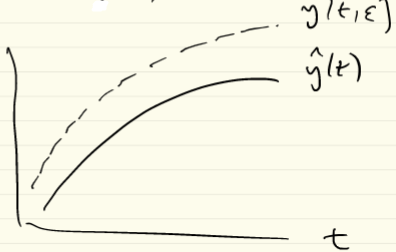
\includegraphics[width=4cm, height=3cm]{pic9}
    \end{center}
    Similarly, let $x(t, \varepsilon) = \widehat{x}(t) + \varepsilon P_{x}(t)$ where $P_{x}(t)$ denotes the corresponding perturbation to $\widehat{x}(t)$ when $\widehat{y}(t)$ is varied according to $P_{y}(t)$. Note that the sum of the perturbations is the variation around the optimum. Define the 'perturbed' lagrangian function as
    \begin{gather*}
    \mathcal{L}(\varepsilon) = \int_{0}^{t_{1}} \left\{ f(t,x(t,\varepsilon),y(t,\varepsilon)) + \mu(t)g(t,x(t,\varepsilon),y(t,\varepsilon)) + \dot{\mu}(t) x(t,\varepsilon) \right\} \ \ dt - \mu(t_{1})x(t_{1}, \varepsilon)+\mu(0)x_{0}
    \end{gather*}
    Recall that $\mathcal{L}$ is maximized at $\widehat{x},\widehat{y}$, where the marginal gain from increasing $\varepsilon$ (ie the perturbation) is 0, and therefore we must have
    \begin{gather*}
    \tfrac{\partial \mathcal{L}(\varepsilon)}{\partial \varepsilon} | (\varepsilon, x, y) = (0, \widehat{x}, \widehat{y}) = 0
    \end{gather*}
    Using the definitions of $x(t,\varepsilon)$, $y(t,\varepsilon)$, and $\mathcal{L}$ the above equation can be expressed as:
    \begin{align*}
     0 = &\int_{0}^{t_{1}} \Big\{ \overbrace{f_{x}(t,\widehat{x}(t),\widehat{y}(t)) + \mu(t)g_{x}(t,\widehat{x}(t),\widehat{y}(t))}^{ \begingroup\color{magenta} H_{x}(t,\widehat{x}(t), \widehat{y}(t), \mu(t)) \endgroup} + \dot{\mu}(t) \Big\} P_{x}(t) \ \ dt \\ &+ \int_{0}^{t_{1}} \underbrace{\Big\{f_{y}(t,\widehat{x}(t), \widehat{y}(t)) + \mu(t)g_{y}(t,\widehat{x}(t), \widehat{y}(t)) \Big\} }_{\begingroup\color{magenta}H_{y}(\cdot)\endgroup} P_{y}(t) \ \ dt - \mu(t_{1})P_{x}(t_{1})
    \end{align*}
    \begin{itemize}
        \item  \underline{Note}: this expression can only hold for all feasible perturbation paths $(P_{x}, P_{y})$ if each integrand vanishes and $\mu(t_{1}) = 0$ such that $P_{y}(t)$ and $P_{x}(t)$ equal 0, which are the conditions of the maximum principle
    \end{itemize}
\end{itemize}

\newpage

\section{Enforcement Frictions I - One-Sided}

\vspace{2.5mm}
\par \underline{Overview}: the analysis of contractual arrangements and enforcement frictions aims to rectify conflicts of interest that arise from violations of two assumptions - (1) both parties were perfectly committed to the rules of the exchange, (2) both parties in the exchange shared the same information. Dropping either of these assumptions creates conflicts of interest
\begin{itemize}
    \item  \underline{Assumption 1 Violation}: here an agent who is not committed to the rules of the exchange would deviate from such rules when she finds it more convenient
    \item  \underline{Assumption 2 Violation}: here an agent who possesses private information would manipulate such information to her advantage
\end{itemize}
\vspace{2.5mm}
\par \underline{Contract Theory}: the study of the economic aspects of contract design where a contract is a set of rules that facilitates cooperation among individuals with conflicting objectives. The goal of contract theory is twofold with the normative goal of how to draw up better contracts and the positive goal of analysing why real life contracts have various forms and designs. We can arbitrarily classify contract theory models by two classifications - (1) according to the type of private information, (2) according to the duration of the contractual relationship
\begin{itemize}
    \item \underline{Type of Private Information}: here we assume that the uninformed party designs the contract and address two types of information issues (adverse selection and moral hazard)
    \begin{itemize}
        \item  \underline{Adverse Selection}: asymmetric information about the characteristics of the informed party (e.g. life insurance where the insured's state of health is unknown by the insurer)
        \item  \underline{Moral Hazard}: asymmetric information about the actions of the informed party (e.g. CEO compensation where the CEO's actions are imperfectly observed by the Board of Directors)
    \end{itemize}
    \item  \underline{Duration of Contractual Relationship}: here we address two types of contract periods (static and dynamic)
    \begin{itemize}
        \item  \underline{Static Contracts}: relationship lasts for one period
        \item  \underline{Dynamic Contracts}: relationship lasts for more than one period (gives rise to enforcement/commitment issues)
    \end{itemize}
\end{itemize}
\vspace{2.5mm}
\par \underline{Principal-Agent Paradigm}: since contracts involve two parties we need to address how the parties bargain over  the terms of the exchange. We bypass the difficulties inherent to the bargaining process by allocating all bargaining power to one of the parties (the Principal) who will offer a take-it or leave-it contract to the Agent. The Principal-Agent Paradigm is the norm in contract theory
\begin{itemize}
    \item \underline{w.l.o.g}: the set of Pareto optimal contracts can be characterised by maximizing the utility of one agent subject to a given level of utility of the other agent. This outcome is a result of the Principal-Agent analogy
\end{itemize}
\vspace{2.5mm}
\par \underline{Enforcement Frictions}: occur when agents are free to walk away from the contract at any time, note that for most models of enforcement frictions we assume that all information is public
\begin{itemize}
    \item  \underline{One-Sided Limited Commitment}: occurs when the principal is committed but the agent is not
    \begin{itemize}
        \item \underline{Applications}: long term labour contracts (principal is the firm and agent is the worker), international lending (principal is the lending country and agent is the borrowing country), firm dynamics (principal is the bank, agent is the entrepreneur seeking to finance a project)
    \end{itemize}
\end{itemize}
\vspace{2.5mm}
\par \underline{Basic Model}: the economy lasts for $T = \infty$ periods and consists of a village with a large number of households. Household preferences are
\begin{gather*}
    U = \mathbb{E}_{0} \sum_{t = 0}^{\infty} \beta^{t} u(c_{t})
\end{gather*}
where $\beta \in (0, 1)$ and $u$ is concave and has the usual properties. \\ \\ Each HH receives a stochastic endowment stream $\left\{y_{t}\right\}_{t=0}^{\infty}$ where $y_{t} \in \left\{ \overline{y}_{1}, \overline{y}_{2}, \dots, \overline{y}_{S} \right\}$ and $\overline{y}_{s+1} > \overline{y}_{s}$. Note that for each $t \geq 0$, $y_{t}$ is independently and identically distributed according to the discrete probability distribution $\Pr(y_{t} = \overline{y}_{s}) = \pi_{s}$ where $s$ is the set from which HHs draw endowments from. At time $t\geq 1$ the household has received a history of endowments $h_{t} = (y_{t}, y_{t-1}, \dots, y_{0})$ \\
\begin{itemize}
    \item \underline{Assumptions}: the endowment processes are iid both across time and across households, overline represents the realizations of the endowments, due to concavity HHs value insurance against endowment realizations, $y_{t}$ is non-storable and therefore self-insruance is precluded
    \item \underline{No Contractual Issue Solution}: if there were a competitive equilibrium with complete markets, at $t=0$ HHs would trade history and date contigent claims before the realization of endowments. Since all HHs are ex ante identical, each HH would end up consuming the per capita endowment in every period and their its lifetime utility would be
    \begin{gather*}
        v_{pool} = \sum_{t=0}^{\infty} \beta^{t} u \Big( \sum_{s=1}^{S} \Pi_{s} \overline{y}_{s} \Big) = \frac{1}{1-\beta} u \Big( \sum_{s=1}^{S} \Pi_{s}\overline{y}_{s} \Big)
    \end{gather*}
    HHs would thus insure away all of the risk associated with their individual endowment process. However, due to limited commitment and other contractual issues, this allocation is unattainable
\end{itemize}
\vspace{2.5mm}
\par \underline{One-Sided Limited Commitment Contract Issue}: in this case, the HH can only trade with the moneylender and can walk away from the contract. If the HH walks away then the HH consumers their endowment and lives in autarky evermore (i.e. the HH cannot return from autarky). Note that only the HH can break the contract, while the moneylender is fully committed to keeping their promise. Therefore, HHs must be induced not to walk away from the contract via structuring the contract in such a way that it is "self-enforcing" in that HHs prefer to conform to it. \\ \\
This involves a contract between the moneylender and the HH as a sequence of history dependent functions $\left\{c_{t}\right\}_{t=0}^{\infty}$ with $c_{t} = f_{t} (y^{t})$. The contract specifies that in each period the HH contributes her endowment realization $y_{t}$ to the moneylender in exchange for consumption $c_{t}$. \\ \\
From this arrangement, the moneylender earns an ex ante expected present value
\begin{gather*}
    P = \mathbb{E}_{0} \sum_{t=0}^{\infty} \beta^{t} (y_{t} - c_{t})
\end{gather*}
where $(y_{t} - c_{t})$ is the net transfer from HH at time t. The moneylender seeks to maximize the expected present value of profits from making contracts. \\ \\
Given the HHs preferences in the basic model, the contract assigns the HH an expected present value of
\begin{gather*}
    v = \mathbb{E} \sum_{t=0}^{\infty} \beta^{t} u(c_{t})
\end{gather*}
If the HH walks away from the contract, the ex ante value associated with consuming the endowment stream in autarky is
\begin{gather*}
    v_{aut} = \mathbb{E}_{0} \sum_{t=0}^{\infty} \beta^{t} u(y_{t}) = \frac{1}{1-\beta} \sum_{s=1}^{S} \Pi_{s} u(\overline{y}_{s})
\end{gather*}
where the continuation utility under autarky is the weighted sum of the possible realizations from the endowment (which due to iid we can remove the dependency of $y$ on time). Note that at time $t$ the HH can guarantee itself a present value of utility of $u(y_{t}) + \beta v_{aut}$ by consuming its own endowment and therefore the moneylender's contract must offer the HH at least this utility at every possible history and every date (this forms the basis of the participation constraint). \\ \\
Here the optimal contract can be analysed using recursive tools, this relies on the inclusion of a participation constraint and promise constraint to entice the HH to stay in the contract
\begin{itemize}
    \item  \underline{Assumptions}: information is symmetric and therefore the moneylender can observe $y_{t}$, the HHs cannot borrow or lend with one another and can only trade with the moneylender, the money lender is risk-neutral and can borrow or lend at the risk free rate $R = \beta^{-1}$, only the money lender has access to the risk-free loan market outside the village, $R$ is exogeneous (i.e. this is a partial equilibrium model)
    \item  \underline{Notation}: our variables include
    \begin{gather*}
    \beta \in (0,1): \ \text{the discount factor} \\
    c_{t}:\ \text{the consumption that the moneylender gives to the HH in exchange for the endowment $y_{t}$ under the contract} \\
    y_{t}:\ \text{the endowment that the HH receives each period} \\
    y^{t}:\ \text{refers to the endowment history up until time t (i.e. the sum of prior endowments)} \\
    \overline{y_{t}}: \ \text{the different possible endowments that could be realized at time $t$}
    w_{t}: \ \text{the sum of the money lender's net gains from each previous period's contract up until time t} \\
    \sum_{s=1}^{S} w_{s}: \ \text{the sum of the money lender's net gains from future periods up until time $S$ given the contracts, where $w_{s}$ refers to the net gain from the contract in a single future period $s$} \\
    v_{aut}: \ \text{the sum of future endowments (as utility) that the HH receives if living in autarky} \\
    v_{t}: \ \text{the discounted sum of future gains (as utility) that the HH receives under the contract from time $t$ onwards, if $t$ is not specified it refers to the present time onwards} \\
    s: \ \text{refers to the state at future time periods}
    \end{gather*}
    Note that the essential difference between $v_{t}$ and $w_{t}$ is that $v$ is the HHs received utility from the contract $u(c_{t})$ and $w_{t}$ is the moneylender's utility gain from the contract $\Pi[y_{t} - c_{t}]$
    \item  \underline{HH "Forward-Looking" State Variable}: note that for the HH, under the contract, the state variable is the promised expected discounted future value (i.e. the sum of all future earnings from the contract). In otherwords, the HH's state variable $v_{t}$ is a "forward-looking" variable where  $v_{t} = \mathbb{E}_{0} \sum_{j=0}^{\infty} \beta^{j} u(c_{t+j})$. This "forward-looking" variable summarizes a stream of future utilities
    \item \underline{Moneylender "Backward-Looking" State Variable}: note that for the moneylender, under the contract, the state variable is the total net gain $(y- c)$ at time $t$. In otherwords, the moneylender's state variable $w_{t}$ is a "backward-looking" variable where $w_{t} = \sum_{t=0}^{t=T} (y_{t} - c_{t})$ (i.e. $w_{t}$ encodes all history dependence in the contract)
    \begin{itemize}
        \item \underline{Logic}: to see how this works, consider the following way of representing a contract $\left\{ f_{t} \right\}$ in terms of a state variable $x_{t}$:
        \begin{align*}
            c_{t} &= g(x_{t}) \\
            x_{t+1} &= \mu (x_{t}, y_{t})
        \end{align*}
        Here $g$ and $\mu$ are time-invariant functions. Notice that by iterating the $\mu(\cdot)$ function $t$ times starting from $(x_{0}, y_{0})$, one obtains
        \begin{gather*}
            x_{t} = m_{t}(x_{0}; y_{t-1}, \dots, y_{0}), \ \ \ t \geq 1
        \end{gather*}
        This allows one to summarize large dimensional shocks and rewards into a single variable and thus $x_{t}$ summarizes histories of endowments
    \end{itemize}
    \item \underline{Participation Contraint}: since autarky is the outside option of the agents, the optimal contract must satisfy the participation constaints where the value of the contract is worth more than the value of autarky and is therefore "self-enforcing" (otherwise the HH will default). Since the money lender arrives at period $y$ before $y_{t}$ is realized and having previously made promised value $v_{t}$ our participation constraint is:
    \begin{gather*}
        u(\overbrace{f_{t}(y^{t})}^{\begingroup\color{magenta} c_{t} \endgroup}) + \underbrace{\beta \mathbb{E}_{t} \sum_{j=1}^{\infty} \beta^{j-1} u(\overbrace{f_{t+j}(y^{t+j})}^{\begingroup\color{magenta} c_{t+j} \endgroup})}_{\begingroup\color{magenta} w_{t}(y^{t}): \ \text{continuation utility at t} \endgroup} \geq u(y_{t}) + \beta v_{aut}
    \end{gather*}
    for all $t, y^{t}$ \\
    We can rewrite our participation constraints can be written as
    \begin{gather*}
        u(f_{t}(y^{t})) + \beta \begingroup\color{cyan} w_{t}(y^{t}) \endgroup \geq u(y_{t}) + \beta v_{aut}
    \end{gather*}
    for all $t, y^{t}$ where
    \begin{gather*}
        \begingroup\color{cyan} w_{t}(y^{t}) \endgroup \equiv \mathbb{E}_{t} \sum_{j=1}^{\infty} \beta^{j-1} u(f_{t+j} (y^{t+j}))
    \end{gather*}
    is the continuation utility of the agent at time $t$, given endowment history $y^{t}$
    \item  \underline{Promise Keeping Constraint}: the Promise Keeping Constraint states that the amount the HH gets in expectation must be greater than $v$, in other words the moneylender must be able to fulfil the contract such that
    \begin{gather*}
        \sum_{s=1}^{S} \Pi_{s} [u(c_{s}) + \beta w_{s}] \geq v
    \end{gather*}
    this renders the planning problem time-consistent with $w_{t}$ encoding the received endowments from the contracts history
    \item  \underline{Moneylender Problem}: each period the money lender chooses how much to give to the HH and how much that they will promise to transfer in the future (which is encoded in $w_{s}$) in order to make the contract "self-enforcing". Here the moneylender chooses $c_{s}$ and a promised value starting in the next time period $v$. Therefore, the the money lender solves
    \begin{gather*}
        P(v) = \max_{\left\{ c_{s}, w_{s} \right\} } \sum_{s=1}^{S} \Pi_{s} [\overline{y}_{s} - c_{s} + \beta P(w_{s})]
    \end{gather*}
    subject to
    \begin{align*}
        \sum_{s=1}^{S} \Pi_{s} [u(c_{s}) + \beta w_{s}] \geq v & \rightarrow \ \text{Promise Keeping Constraint} \\
        u(c_{s}) + \beta w_{s} \geq u(\overline{y}_{s}) + \beta v_{aut}, \ \ s = 1, \dots, S & \rightarrow \ \text{Participation Constraint}
    \end{align*}
    Here $w_{s} \in [v_{aut}, \overline{v}]$ where $\overline{v}$ is a large number. $w_{s}$ is the \textit{future} (i.e. next period) realized transfer under the contract established at time $s$, given that $y = \overline{y}_{s}$ this period. $w_{s}$ therefore represents the promised value which the HH will enter next period). We treat promised utility $v$ as a state variable for the HH. Note that $P$ must be a decreasing function of $v$ because the higher the consumption stream of the villager, the lower must be the profits of the moneylender
    \begin{itemize}
        \item  \underline{Characterisation}: it can be shown that the constraint set is convex and that the value function $P(v)$ is stictly concave (as well as differentiable). Given this we have the following lemmas that essentially state that agents have incentives to walk away when income realisations are large enough - wherein the participation constraint will bind for a $\overline{y}_{s}$ that is significantly high.
        \begin{itemize}
            \item \underline{Lemma 1}: for each $v$, there exists a threshold $\overline{y}(v)$ such that the PC binds binds if and only if $\overline{y}_{s} \geq \overline{y}(v)$
            \begin{itemize}
                \item  \underline{Logic}: in other words, for every possible "discounted sum of future gains", there exists a theshold endowment level such that the PC will bind if the actual endowment level is greater or equal to the figurative endowment level. This makes sense, since if the HH receives a particularly high endowment this period then the moneylender will offer distribute $y_{t}$ with a lower proportion of $u(c_{t})$ and a higher proportion $c_{t+j}$ to make the contract "self-enforcing"
            \end{itemize}
            \item  \underline{Lemma 2}: the threshold $\overline{y}(v)$ is increasing in v
            \begin{itemize}
                \item  \underline{Logic}: this makes sense since a higher $v$ occurs when $c_{s+j}$ increases. $c_{t+j}$ increases when $\overline{y}(v)$ is reached, with the moneylender offering a lower proportion (relative to $y_{s}$) of $u(c_{t})$ as part of the contract (though $u(c_{t})$ will still be higher than when receiving $y_{1} < y_{s}$)
            \end{itemize}
            \item  \underline{Proof}: we write the lagrangian as
            \begin{gather*}
                \mathcal{L} = \sum_{s=1}^{S} \Pi_{s} [\overline{y}_{s} - c_{s} + \beta P(w_{s})] \\ + \varepsilon \left\{ \sum_{s=1}^{S} \Pi_{s} [u(c_{s}) + \beta w_{s} - v \right\} \\ +  \sum_{s=1}^{S} \eta_{s} \left\{ u(c_{s}) + \beta w_{s} - u(\overline{y}_{s}) - \beta v_{aut} \right\}
            \end{gather*}
            where $\varepsilon$ and $\eta$ are the lagrangian multipliers on the Promise Keeping Constraint and Participation Contraint respectively. Taking first order conditions and applying the envelope theorem yields the following:
            \begin{align*}
                \frac{\partial \mathcal{L}}{\partial C_{s}} = 0 &\rightarrow -\Pi_{s} + \varepsilon \Pi_{s} u^{'}(C_{s}) + \eta_{s} u^{'} (C_{s}) = 0 \tag{1} \\
                \frac{\partial \mathcal{L}}{\partial w_{s}} = 0 &\rightarrow \eta_{s} + \varepsilon \Pi_{s} = - \Pi_{s}P^{'}(w_{s}) \tag{2} \\
                \text{Envelope Theorem}: \ \ &\rightarrow P'(v) = - \varepsilon < 0 \tag{3}
            \end{align*}
            Rearranging equations $(1)$ and $(2)$ for $\varepsilon \Pi_{s} + \eta_{s}$ and solving them simultaneously yields
            \begin{align*}
                u^{'}(C_{s}) = - P^{'}(w_{s})^{-1} \tag{4}
            \end{align*}
            It is clear to see that the LHS of this equation falls with $C_{s}$ due to concavity of $u(\cdot)$ and the RHS of this equation falls with $w_{s}$ due to concavity of $P(\cdot)$. This implies that $C_{s}$ and $w_{s}$ are positively related. In otherwords, as our lemma states, a higher $C_{s}$ results in a higher $w_{s}$ since the moneylender will provide lower levels of $C_{s+j}$
            \newline
            Combining $(3)$ and $(2)$ yields the law of motion for continuation Utility
            \begin{align*}
                P^{'}(w_{s}) = P^{'}(v) - \frac{\eta_{s}}{\Pi_{s}} \tag{5}
            \end{align*}
            \newline
            \underline{Lemma 1 Proof}
            \newline
            Take as given that $\overline{y}_{s}$ subject to PC is not binding (i.e. $\eta_{s} = 0$), therefore by $(5)$ we have
            \begin{gather*}
                P^{'}(w_{s}) = P^{'}(v) \Rightarrow w_{s} = v \ \ \text{by concavity}
            \end{gather*}
            Using this fact into $(4)$ we can write $c$ as a function of only $v$ and so have
            \begin{gather*}
                u^{'}(C_{s}) = -P^{'} (v)^{-1}
            \end{gather*}
            Which can be rewritten as $C_{s} = g_{1}(v), \ \ g_{1}^{'} > 0$. This allows us to rewrite the PC as
            \begin{gather*}
                u(C_{s}) + \beta w_{s} > u(\overline{y}_{S}) + \beta v_{aut} \\
                \Big\Downarrow \\
                u(g_{1}(v)) + \beta v > u(\overline{y}) + \beta v_{aut} \equiv \overline{y}(v) \\
                \Big\Downarrow \\
                \underbrace{u^{-1} (u(g_{1}(v)) _ \beta (v-v_{aut}))}_{\begingroup\color{cyan} \equiv \overline{y}(v) \endgroup} > \overline{y_{s}}
            \end{gather*}
            Thus, given the definition of $\overline{y}(v)$, the PC is not binding if and only if $\overline{y}_{s} < \overline{y}(v)$
            \newline
            \underline{Lemma 2 Proof}
            \newline
            Given the definition of $\overline{y}(v)$ from the proof for Lemma 1, this is straightforward
                \newline
                \begin{center}
                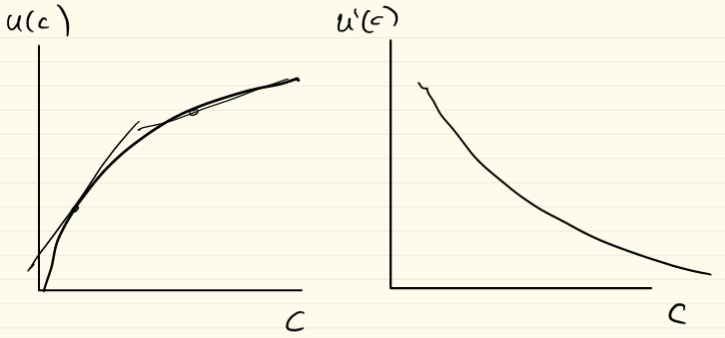
\includegraphics[width=4cm, height=3cm]{pic11}
                \end{center}
        \end{itemize}
    \end{itemize}
    \item \underline{Properties of PC Binding vs Not Binding}
    Suppose PC is not binding, then $w_{s} = v$ and $C_{s} = g_{1}(v)$ where $g_{1}^{'} > 0$. Therefore, if PC is not binding then $w_{s}$ and $C_{s}$ remain constant with consumption in state $s$ depending on promised utility $v$ but not on the endowment in state $s$ \\ \\
    Suppose PC is binding, then $w_{s} = l(\overline{y}_{s}) > v$ and $C_{s} = g_{2}(\overline{y}_{s}) \in (g_{1}(v), \overline{y}_{s})$ where $l^{'}, g_{2}^{'} \geq 0$. \\ \\ Therefore, if PC is binding then $w_{s}$ and $C_{s}$ must increase to induce the agent not to walk away from the contract - wherein $w_{s}$ and $c_{s}$ only depend on current income realisations (and not on the history of shocks given by $v$)
    \begin{itemize}
        \item \underline{Consumption under Optimal Contract}: graphically, given v, consumption under the optimal contract is
            \newline
            \begin{center}
            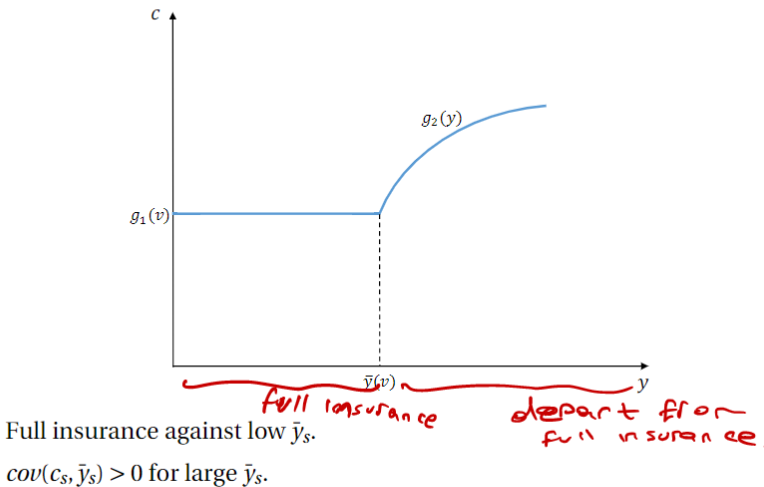
\includegraphics[width=8cm, height=6cm]{pic12}
            \end{center}
        \item \underline{Long Run Dynamics}: $c_{t}$ increases over time until $\overline{y}_{S}$ is realized
            All agents eventually become fully insured (no fluctuations in consumptions) when their highest income realization $\overline{y}_{S}$ is realized and therefore $C$ eventually becomes constant.
            \newline
            \begin{center}
            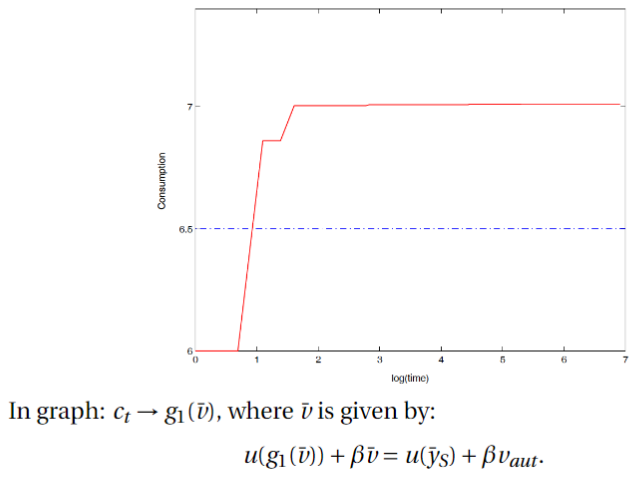
\includegraphics[width=8cm, height=6cm]{pic13}
            \end{center}
            With many HHs, all agents eventually get to consume $g_{1}(\overline{v})$: $\lim_{t \rightarrow \infty} \Pr(c_{t} = g_{1}(\overline{v})) = 1$. Overall, we have "fanning in" of the cross-sectional distribution of consumption and full risk sharing in the long run (ie t=500)
            \newline
            \begin{center}
            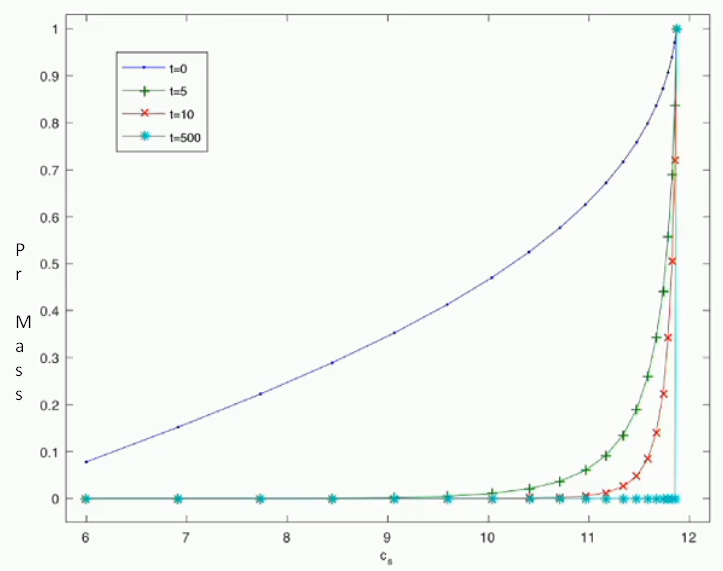
\includegraphics[width=8cm, height=6cm]{pic14}
            \end{center}
        \item  \underline{Not Binding Proof}: shown in the proof of the lemma
        \item  \underline{Binding Proof}: assume that PC is binding
        \begin{itemize}
            \item \underline{Step 1}: show that $w_{s}$ and $c_{s}$ are only functions of $\overline{y}_{s}$
            \newline
            By FOC $(4)$ we have $u^{1} (C_{s}) = -P^{'}(w_{s})^{-1}$ and given the fact that PC is binding we have $u(C_{s}) + \beta w_{s} = u(\overline{y}_{s}) + \beta v_{aut}$. Note that these two equations form a system of 2 equations in 2 unknowns ($C_{s}, w_{s}$). Since promised $v$ does not show up in this system we can write its solution as $w_{s} = \mathcal{l}(\overline{y}_{s})$ and $C_{s} = g_{2}(\overline{y}_{s})$
            \item  \underline{Step 2}: show that $g_{2}^{'} > 0$ and $\mathcal{l}^{'} > 0$
            \newline
            By $u(C_{s}) + \beta w_{s} = u(\overline{y}_{s}) + \beta v_{aut}$ we know that $[u(C_{s}) + \beta w_{s}]$ is non-decreasing in $\overline{y}_{s}$. Also, by $u^{1} (C_{s}) = -P^{'}(w_{s})^{-1}$ (as shown previously), $C_{s}$ is non-decreasing in $w_{s}$ and hence $C_{s}$ should be non-decreasing in $\overline{y}_{s}$
            \item  \underline{Step 3}: show that $w_{s} > v$
            \newline
            By $P^{'}(w_{s}) = P^{'}(v) - \tfrac{\eta_{s}}{\Pi_{s}}$, if the PC binds then $\eta_{s} > 0$ and so $P^{'}(w_{s}) < P^{'}(v) \Rightarrow w_{s} > v$ via concavity
            \item  \underline{Step 4}: show that $C_{s} \in (g_{1}(v), \overline{y}_{s})$
            \newline
            A binding PC implies that $u(C_{s}) + \beta w_{s} = u(\overline{y}_{s}) + \beta v_{aut}$. Therefore, $c_{s} < \overline{y}_{s}$. Because $w_{s} > v$ we have
            \begin{gather*}
                -P^{'}(w_{s})^{-1} < -P^{'}(v)^{-1} \\
                \Big\Downarrow \\
                u^{'}(C_{s}) < u^{'}(g_{1}(v)) \ \ \text{by (4)} \\
                \Big\Downarrow \\
                C_{s} > g_{1}(v)
            \end{gather*}
        \end{itemize}
    \end{itemize}
    \item \underline{Connection to Labour Contracts}: early work on one-sided limited commitment models aimed at analysing the characteristics of labour contracts. In our model this can be mapped as $C$ being the wage offered within a firm, $y$ shock being wages offered in the spot market, and the enforcement friction being labour mobility. Since workers are risk-averse, they value insurance against fluctuations in the spot market for wages (i.e. implicit insurance premium in contractual wages). Firms find contractual arrangement beneficial because in the short run they can pay wages below those in the spot market (due to the implicity insurance premium), which is embedded by $C_{s} < \overline{y}_{s}$ when PC binds in our model
\end{itemize}

\newpage

\section{Enforcement Contracts II - Two-Sided}

\vspace{2.5mm}
\par \underline{Overview}: two agents "share risk" if they use state-contingent transfers to increase the expected utility of both, by reducing the risk of at least one. In the absence of contractual frictions there should be full risk sharing with all idiosyncratic risk eliminated and only aggregate risk affecting individuals' consumption. However, despite this we find that, even after conditioning for aggregate income, individual income is positively correlated with current and lagged individual income (i.e. risk is not shared across time). This inconsistency has three causes.
\begin{itemize}
    \item  \underline{Cause 1 - Exogeneously Incomeplete Markets}: occurs when there are more states than assets and therefore transferring wealth across certain is restricted. For example, in Bewley-Hugget-Aiyagari models agents can only use a single bond to insure against idiosyncratic labour income shocks. However, this involves assuming that some asset markets are shut down - such as through arbitray assumptions about which assets are available (conclusions are sensitive to these assumptions)
    \item  \underline{Cause 2 - Private Information Frictions}: occurs when consumption is correlated with individual income to induce truth-telling or adequate efforce. This involves two major drawbacks:
    \begin{itemize}
        \item  \underline{Drawback 1 - Imperfect Risk Sharing}: holds event in environments where informational asymmetries are small (e.g. village economies or within families)
        \item  \underline{Drawback 2 - Longrun Implications of Private Infomration}: these models are counterfactual
    \end{itemize}
    \item  \underline{Cause 3 - Two-sided Limited Commitment}: occurs when there is an optimal insurance arrangement between two agents who lack commitment. This differs from one-sided limited commitment (where agents can default but principals cannot) in that both the principal and the agent can default. The key results of modelling two-sided limited commitment are that incomeplete risk sharing can be perpetual and the amount of risk sharing endogenously emanates from limited enforcement frictions
\end{itemize}
\vspace{2.5mm}
\par \underline{Kocherlakota Model of Two-sided Limited Commitment}: involves two infinitely-lived agents subject to endowment shocks where the state of the world is determined by realization of $\theta_{t} \in \left\{ 1, \dots, S \right\}$, which is iid with $\Pr (\theta_{t} = s) = \pi_{s} > 0$. In other words, the endowment profile of the agents, $(y_{t}^{1}, y_{t}^{2})$ is determined by realization of $\theta_{t}$.
The aggregate endowment is $Y_{t} = y_{t}^{1} + y_{t}^{2} \geq 0$ and the joint distribution of endowments is symmetric such that $\Pr(y, y^{'}) = \Pr(y', y)$ \footnote{a special case occurs where there is no aggregate uncertainty (i.e. $Y_{t} = 1$), $\theta_{t} \in [0,1]$, $y_{t}^{1} = \theta_{t}, \ y_{t}^{2} = 1 - \theta_{t}$, and the distribution of $\theta_{t}$ is symmetric around 1/2}.
Given identical preferences, both agents have the following objective function
\begin{gather*}
\mathbb{E}_{0} \sum_{t=1}^{\infty}\beta_{t-1}u(c_{t})
\end{gather*}
where $\beta \in (0,1)$, u is increasing, strictly concave, and differentiable.
An allocation $\textbf{c} = \left\{ c_{t}^{j}\right\}_{t=1, j=1}^{\infty, 2}$ is feasible if and only if $$c_{t}^{1} + c_{t}^{2} \leq Y_{t}$$ for all $t = 1, 2, \dots, \infty$
\begin{itemize}
    \item  \underline{Assumptions}: there is no outside lender (agents can only contract with other agents)
    \item \underline{Contract}: agents sign a contract to insure against endowment shocks and each agent can walk away from the contract at time $t$. Agents proceed with the following steps per period
    \begin{itemize}
        \item  \underline{Step 1}: $\theta_{t}$ is realized and therefore $(y_{t}^{1}, y_{t}^{2})$ is observed by both agents
        \item  \underline{Step 2}: each individual $j$ simultaneously transfers $TR_{t}^{j} = y_{t}^{j} - c_{t}^{j}$ to the other
    \end{itemize}
    \item  \underline{Autarky}: if an agent defaults, they live in autark forever with utility
    \begin{gather*}
        v_{aut} = \sum_{s=1}^{S} \pi_{s} \big[ u(y_{s}^{j}) + \beta V_{aut} \big]
    \end{gather*}
    Note that the symmetry of distribution of $(y_{t}^{1}, y_{t}^{2})$ guarantees that $v_{aut}^{1} = v_{aut}^{2}$
    \item  \underline{Participation Constraints} in order to induce participation and prevent an agent from defaulting the following participation constraint must hold
    \begin{gather*}
        u(c_{t}^{j}) + \mathbb{E}_{t}\sum_{\tau = 1}^{\infty} \beta^{\tau}u(c_{t+\tau}^{j}) \geq u(y_{t}^{j}) + \beta V_{aut}, \ \ \ j = 1,2
    \end{gather*}
    for all dates and states.
    Note that an allocation $\textbf{c}$ is sustainable if it is feasible and satisfies participation constraints
    \item  \underline{Efficient Allocations}: a sustainable allocation $\textbf{c}$ is efficient if there is no other sustainable allocation providing both individuals with at least as much utility and one individual with more (i.e. an efficient allocation is Pareto Optimal)
    \item  \underline{Contract Design with a Principal and an Agent}: efficient allocations can be found by solving the planning problem
    \begin{gather*}
        V(w) = \max_{c_{s}, w_{s}} \sum_{s=1}^{S} \pi_{s} \big[u(Y_{s} - c_{s}) + \beta V(w_{s})\big] \\
        \text{s.t:} \ \ \sum_{s=1}^{S} \pi_{s} [u(c_{s}) + \beta w_{s}] = w \tag{$PK_{c}$}\\
        u(c_{s}) + \beta w_{s} \geq u(y_{s}^{1}) + \beta V_{aut}, \ \ \ \forall s \tag{$PC^{1}$} \\
        u(Y_{s} - c_{s}) + \beta V(w_{s}) \geq u(Y_{s} - y_{s}^{1}) + \beta V_{aut}, \ \ \ \forall s \tag{$PC^{2}$}
    \end{gather*}
    where $w \in [V_{aut}, V_{max}]$
    Note that $(c_{s}, w_{s})$ are the consumption and continuation utility allocations of Agent 1 given state s, $(Y_{s} - c_{s}, V(w_{s}))$ are the consumption and continuation utility allocations of Agent 2 given state s, and $V(w)$ represents the Pareto frontier (traced out by changing $w$)
    \newline
    \begin{center}
    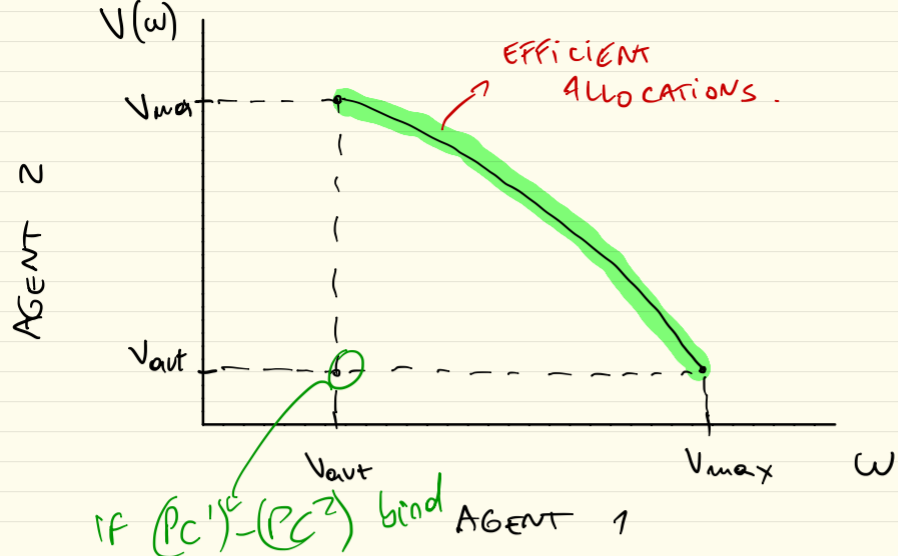
\includegraphics[width=8cm, height=6cm]{pic16}
    \end{center}
    \begin{itemize}
        \item  \underline{First Best Allocation} for the first best allocation there is full risk sharing and we solve
        \begin{gather*}
            V(w) = \max_{c_{s}, w_{s}} \sum_{s=1}^{S} \pi_{s} [u(Y_{s} - c_{s}) + \beta V(w_{s})] \\
            \text{s.t:} \ \ \sum_{s=1}^{S} \pi_{s} [u(c_{s}) + \beta w_{s}] = w
        \end{gather*}
        \begin{itemize}
            \item  \underline{Proof}: writing the Lagrangian we have
            \begin{gather*}
                \sum_{s=1}^{S} \pi_{s} [u(Y_{s} - c_{s}) + \beta V(w_{s})] - \lambda \left\{\sum_{s=1}^{S} \pi_{s} [u(c_{s}) + \beta w_{s}] - w \right\}
            \end{gather*}
            The FOCs of the First Best Allocation includes:
            \begin{gather*}
                \frac{\partial \lambda}{\partial c} = 0 \Rightarrow -\Pi_{s}u^{'}(Y_{s} - c_{s}) + \lambda \Pi_{s} u^{'}(c_{s}) = 0 \\
            \end{gather*}
            Rearranging this we have
            \begin{gather*}
                \frac{u^{'}(Y_{s} - c_{s})}{u^{'}(c_{s})} = \lambda
            \end{gather*}
            This implies full risk sharing with individual consumption only function with average income
        \end{itemize}
        The solution will be driven by the pattern of binding PCs wher ethe possible stated of the world can be divided into four groups
        \begin{itemize}
            \item  \underline{State 1}: in which $PC_{1}$ binds
            \item  \underline{State 2}: in which $PC_{2}$ binds
            \item  \underline{State 3}: in which neither $PC$ binds
            \item  \underline{State 4}: in which both $PCs$ bind
        \end{itemize}
        Since state 4 never holds if the allocation is efficient only state 1-3 are possibilities
        \begin{itemize}
            \item  \underline{Proof}: suppose that $PC_{1}$ is binding, then $u(c_{s}) + \beta w_{s} = u(y_{s}^{'}) + \beta v_{aut}$. This implies that $c_{s} \leq y_{s}^{1}$ since $w_{s} \geq v_{aut}$
            Suppose that $PC_{2}$ is binding, then $u(Y_{s} - c_{s}) + \beta v(w_{s}) = u(y_{s}^{2}) + \beta v_{aut}$. This implies the following:
            \begin{align*}
                u(Y_{s} - c_{s}) - u(y_{s}^{2}) &= \beta \overbrace{[v_{aut} - v(w_{s})]}^{\leq 0} \\
                u(y_{s} - c_{s}) &\leq u(y_{s}^{2}) \\
                u(Y_{s} - c_{s}) &\leq u(Y_{s} - Y_{s}^{1}) \\
                Y_{s} - c_{s} &\leq Y_{s} - Y_{s}^{1}
            \end{align*}
            Therefore $c_{s} \geq y_{s}^{1}$. \\ \\
            This means that if both participation constraints bind we have $PC^{1} \rightarrow c_{s} \leq y_{s}^{1}$ and $PC^{2} \rightarrow c_{s} \geq y_{s}^{1}$, therefore $c_{s} = y_{s}^{1}$. This implies that $w_{s} = v_{aut}$ and $v(w_{s}) = v_{aut}$, thus both $PCs$ binding is not an efficient solution
        \end{itemize}
        \item \underline{Efficient Allocations}: it can be shown that V is differentiable, decreasing, and concave. This implies the following evolution of promised utility given our states:
        \begin{itemize}
            \item  \underline{State 1 Evolution}: if $PC_{1}$ binds then $w_{s} > w$
            \item  \underline{State 2 Evolution}: if $PC_{2}$ binds then $w_{s} < w$
            \item  \underline{State 3 Evolution}: if neither $PC$ binds then $w_{s} = w$
        \end{itemize}
        This means that, unlike with one-sided commitment, promised values can fall.
        \begin{itemize}
            \item  \underline{Proof}: we have the following objective function
            \begin{gather*}
                v(w) = \max_{c_{s}, w_{s}} \sum_{s} \Pi_{s} [u(y_{s} - c_{s}) + \beta v(w_{s})] \\
                \text{s.t:} \ \ \sum_{s} \Pi_{s}[u(c_{s}) + \beta w_{s}] = w \tag{$\eta$} \\
                u(c_{s}) + \beta w_{s} \geq u(y_{s}^{'}) + \beta v_{aut}, \ \ \ \forall s \tag{$\mu_{s}^{1}$} \\
                u(Y_{s} - c_{s}) + \beta v(w_{s}) \geq u(y_{s}^{2}) + \beta v_{aut}, \ \ \ \forall s \tag{$\mu_{s}^{2}$} \\
            \end{gather*}
            Taking first order conditions and applying the envelope theorem yields the following:
            \begin{align*}
             \frac{\partial v}{\partial w_{s}} = 0 &\rightarrow \Pi_{s} \beta v^{'}(w_{s}) + \eta \Pi_{s} \beta + \mu_{s}^{1} \beta + \mu_{s}^{2} \beta V^{'}(w_{s}) = 0 \tag{1} \\
             \frac{\partial v}{\partial c_{s}} = 0 &\rightarrow - \Pi_{s}u^{'}(Y_{s} - c_{s}) + \eta \Pi_{s}u^{'}(c_{s}) + \mu_{s}^{1}u^{'}(c_{s}) - \mu_{s}^{2} u^{'}(y_{s} - c_{s}) = 0 \tag{2} \\
             \text{Envelope Theorem} &\rightarrow v^{'}(w) = -\eta \tag{3}
         \end{align*}
            We need to consider the 3 states: (1) when $PC_{1}$ binds and therefore $\mu_{s}^{1} > 0, \  \mu_{s}^{2} = 0$, (2) when $PC_{2}$ binds and therefore $\mu_{s}^{1} = 0, \ \mu_{s}^{2} > 0$, (3) no PC binds and therefore $(\mu_{s}^{1} = \mu_{s}^{2} = 0)$
            \begin{itemize}
                \item  \underline{State 1 - $PC_{1}$ Binds}: by $(1)$ and $(3)$ we have
                \begin{gather*}
                    \Pi_{s}v^{'}(w_{s}) \sout{\beta} - v^{'}(w) \Pi_{s} \sout{\beta} + \mu_{s}^{1} \sout{\beta} = 0 \\
                    \big\Updownarrow \\
                    v^{'}(w_{s}) = v^{'}(w) - \frac{\mu_{s}^{1}}{\Pi_{s}}
                \end{gather*}
                Therefore $v^{'}(w_{s}) < v^{'}(w)$ and thus, by concavity, $w_{s} > w$
                \item  \underline{State 2 - $PC_{2}$ Binds}: by rearranging equations $(1)$ and $(3)$ we get
                \begin{gather*}
                    v^{'}(w_{s}) = \frac{\Pi_{s}}{\Pi_{s} + \mu_{s}^{2}} v^{'}(w) \\
                    \Downarrow \\
                    \frac{v^{'}(w_{s})}{v^{'}(w)} = \frac{\Pi_{s}}{\Pi_{s} + \mu_{s}^{2}} < 1 \\
                    \Downarrow \\
                    v_{'}(w_{s}) > v^{'}(w)
                \end{gather*}
                Therefore, $w_{s} < w$
                \item  \underline{State 2 - No PC Binds}: by $(1)$ and $(3)$ we have that $v^{'}(w_{s}) = v^{'}(w)$. Therefore, $w_{s} = w$
            \end{itemize}
        \end{itemize}
        Analogously to what we showed in the one-sided limited commitment model, it follows that:
        \begin{itemize}
            \item  $PC_{1}$ binds when $y_{s}^{1}$ is high
            \item  $PC_{2}$ binds when $y_{s}^{2}$ is high
            \item  $w_{s}$ is a non-decreasing function of $c_{s}$
        \end{itemize}
        Combined with the evolution of promised utilitys this implies that $Cov(c_{t}, y_{t} | Y_{t}) \geq 0$ and therefore we have imperfect risk sharing. Given the correlation result with imperfect risk sharing, lagged individual income occurs since in an efficient allocation $$Cov(c_{t}^{j}, y_{t-k}^{j} | Y_{t-k}) \geq 0$$ for $k \geq 0$ and $j = 1,2$
        \item \underline{Long-Run Dynamics}: suppose the first best allocation is not sustainable. Then as $t \rightarrow \infty$, $\Pr(w_{t} | w_{0})$ converges in distribution to the same non-degenerate limiting distribution for all $w_{0}$.
        As a result the first best is typically not sustainable whenever $\beta$ is small enouggh. This result strengthens the previous result on imperfect risk sharing in two dimensions:
        \begin{itemize}
            \item  \underline{Dimension 1}: it holds in the long run, as the limiting distribution is non-degenerate
            \item  \underline{Dimension 2}: the same distribution (and hence correlation) is obtained regardless of initial promised values
        \end{itemize}
    \end{itemize}
\end{itemize}
\underline{Graphical Intuition for Perpetual Imperfect Risk Sharing}
\begin{center}
\textbf{One Sided Limited Commitment} \par
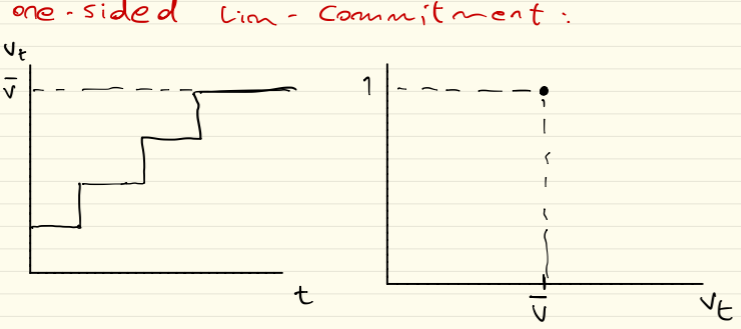
\includegraphics[width=4cm, height=3cm]{pic17}
\end{center}
\begin{center}
\textbf{Two Sided Limited Commitment} \par
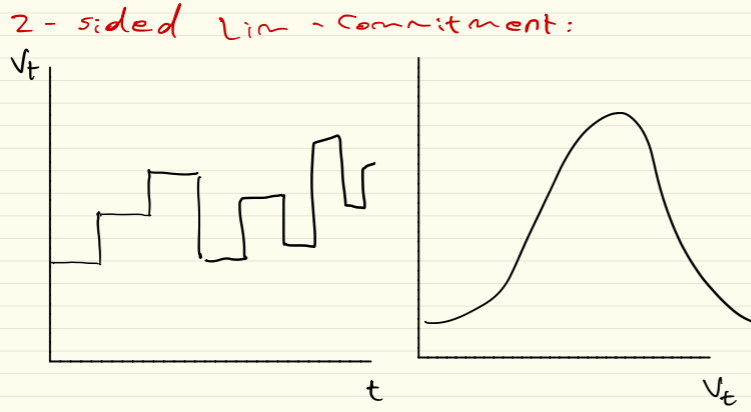
\includegraphics[width=4cm, height=3cm]{pic18}
\end{center}


\end{document}
